%%%%%%%%%%%%%%%%%%%%%%%%%%%%%%%%%%%%%%%%%%%%%%%%%%%%%%%%%%%%%%%%%%%%%%%%%%%%%%%%
%                         FORMATO DE TESIS Unipamplona                         %
%%%%%%%%%%%%%%%%%%%%%%%%%%%%%%%%%%%%%%%%%%%%%%%%%%%%%%%%%%%%%%%%%%%%%%%%%%%%%%%%
% based on Harish Bhanderi's PhD/MPhil template, then Uni Cambridge
% http://www-h.eng.cam.ac.uk/help/tpl/textprocessing/ThesisStyle/
% corrected and extended in 2007 by Jakob Suckale, then MPI-iCBG PhD programme
% and made available through OpenWetWare.org - the free biology wiki
% forked from https://github.com/lestebanv/plantillalatexup/
% modifications made by Luis Alberto Esteban Villamizar

%                     Under GNU License v3

% ADAPTADO PARA la Universidad de Pamplona:  Luis Alberto Esteban Villamizar

\documentclass[twoside,11pt]{Latex/Classes/thesisUP}
\usepackage[spanish]{babel}
\usepackage{blindtext}                     % Para insertar texto dummy, de ejemplo, pues.
% Note:
% The \blindtext or \Blindtext commands throughout this template generate dummy text
% to fill the template out. These commands should all be removed when 
% writing thesis content.

\usepackage[sort&compress]{natbib}  % Personalizar la bibliografía a gusto de cada quien

% This file contains macros that can be called up from connected TeX files
% It helps to summarise repeated code, e.g. figure insertion (see below).

%%%%%%%%%%%%%%%%%%%%%%%%%%%%%%%%%%%%%%%%%%%%%%
%            Colores de la UNAM              %
%%%%%%%%%%%%%%%%%%%%%%%%%%%%%%%%%%%%%%%%%%%%%%
% Para UNAN: Azul Pantone 541  -->(0,63,119) RGB
% Para UMSNH: PANTONE Blue 072 C
\definecolor{Azul}{RGB}{51,51,153}

% Para UNAM: Oro Pantone 460  -->(234,221,150) RGB
% Para UMNSH: PANTONE 110 C
\definecolor{Oro}{RGB}{204,153,51}


%%%%%%%%%%%%%%%%%%%%%%%%%%%%%%%%%%%%%%%%%%%%%%
%            Comandos para líneas            %
%%%%%%%%%%%%%%%%%%%%%%%%%%%%%%%%%%%%%%%%%%%%%%
%Se define un comando \colorvrule para hacer líneas verticales de color con 3 argumentos: color, ancho, alto
\newcommand{\colorvrule}[3]{
\begingroup\color{#1}\vrule width#2 height#3
\endgroup}

%Se define un comando \colorhrule para hacer líneas horizontales de color con 2 argumentos: color, ancho
\newcommand{\colorhrule}[2]{
\begingroup\color{#1}\hrule height#2
\endgroup}

%%%%%%%%%%%%%%%%%%%%%%%%%%%%%%%%%%%%%%%%%%%%%%
%          Comando para derivadas            %
%%%%%%%%%%%%%%%%%%%%%%%%%%%%%%%%%%%%%%%%%%%%%%
\newcommand{\derivada}[3][]{\ensuremath{\dfrac{\mbox{d}^{#1}#2}{\mbox{d}#3^{#1}}}} 
%primer argumento(opcional): orden de la derivada
%segundo argumento: función a derivar
%tercer argumento: variable respecto a la que se deriva


%%%%%%%%%%%%%%%%%%%%%%%%%%%%%%%%%%%%%%%%%%%%%%
%       Comando para la exponencial          %
%%%%%%%%%%%%%%%%%%%%%%%%%%%%%%%%%%%%%%%%%%%%%%
\newcommand{\e}[1][]{\ensuremath{\mbox{e}^{#1}}}
%primer argumento(opcional): exponente de la exponencial




% insert a centered figure with caption and description
% parameters 1:filename, 2:title, 3:description and label
\newcommand{\figuremacro}[3]{
	\begin{figure}[htbp]
		\centering
		\includegraphics[width=1\textwidth]{#1}
		\caption[#2]{\textbf{#2} - #3}
		\label{condicion}
	\end{figure}
}

% insert a centered figure with caption and description AND WIDTH
% parameters 1:filename, 2:title, 3:description and label, 4: textwidth
% textwidth 1 means as text, 0.5 means half the width of the text
\newcommand{\figuremacroW}[4]{
	\begin{figure}[htbp]
		\centering
		\includegraphics[width=#4\textwidth]{#1}
		\caption[#2]{\textbf{#2} - #3}
		\label{#1}
	\end{figure}
}

% inserts a figure with wrapped around text; only suitable for NARROW figs
% o is for outside on a double paged document; others: l, r, i(inside)
% text and figure will each be half of the document width
% note: long captions often crash with adjacent content; take care
% in general: above 2 macro produce more reliable layout
\newcommand{\figuremacroN}[3]{
	\begin{wrapfigure}{o}{0.5\textwidth}
		\centering
		\includegraphics[width=0.48\textwidth]{#1}
		\caption[#2]{{\small\textbf{#2} - #3}}
		\label{#1}
	\end{wrapfigure}
}

% predefined commands by Harish
\newcommand{\PdfPsText}[2]{
  \ifpdf
     #1
  \else
     #2
  \fi
}

\newcommand{\IncludeGraphicsH}[3]{
  \PdfPsText{\includegraphics[height=#2]{#1}}{\includegraphics[bb = #3, height=#2]{#1}}
}

\newcommand{\IncludeGraphicsW}[3]{
  \PdfPsText{\includegraphics[width=#2]{#1}}{\includegraphics[bb = #3, width=#2]{#1}}
}

\newcommand{\InsertFig}[3]{
  \begin{figure}[!htbp]
    \begin{center}
      \leavevmode
      #1
      \caption{#2}
      \label{#3}
    \end{center}
  \end{figure}
}          % Archivo con funciones útiles



%%%%%%%%%%%%%%%%%%%%%%%%%%%%%%%%%%%%%%%%%%%%%%%%%%%%%%%%%%%%%%%%%%%%%%%%%%%%%%%%
%                                   DATOS                                      %
%%%%%%%%%%%%%%%%%%%%%%%%%%%%%%%%%%%%%%%%%%%%%%%%%%%%%%%%%%%%%%%%%%%%%%%%%%%%%%%%
\title{AUTOMATIZACIÓN Y DIGITALIZACIÓN DE PROCESOS ASIGNADOS POR LOS COLABORADORES DEL BANCO DE BOGOTÁ MEDIANTE LAS HERRAMIENTAS DE MICROSOFT 365 Y POWER PLATFORM}
\author{Sergio Luis López Atencio} 
\director{Luz Marina Santos Jaimes}%  Director del trabajo o Tutor, si aplica
\institucion{Universidad de Pamplona}
\facultad{Facultad de Ingenierías y Arquitectura}                
\escudofacultad{Prologo/imagenes/escudogriseslineas}% Aquí ponen la ruta y nombre del escudo de su facultad
\dept{Eléctrica, Electrónica, Telecomunicaciones y Sistemas}
\programa{PROGRAMA DE INGENIERÍAS DE SISTEMAS} % Programa
\degree{Ingeniero de sistemas}   % Titulo a obtener                                 
\degreedate{2022}% Año de la fecha de la presentacion del trabajo
\lugar{Pamplona, Colombia}% Lugar

%\portadafalse                              % Portada en NEGRO, descomentar y comentar la línea siguiente si se quiere utilizar
\portadatrue                                % Portada en COLOR



\keywords{tesis,Sergio Luis López Atencio,Luz Marina Santos Jaimez,etc}% Palablas clave para los metadatos del PDF
\subject{Trabajo de grado,Power Platform}% Tema para metadatos del PDF  

%%%%%%%%%%%%%%%%%%%%%%%%%%%%%%%%%%%%%%%%%%%%%%%%%%%%%
%                   PORTADA                         %
%%%%%%%%%%%%%%%%%%%%%%%%%%%%%%%%%%%%%%%%%%%%%%%%%%%%%
\begin{document}
	
	\maketitle									% Se redefinió este comando en el archivo de la clase para generar automáticamente la portada a partir de los datos
	
	%%%%%%%%%%%%%%%%%%%%%%%%%%%%%%%%%%%%%%%%%%%%%%%%%%%%%
	%                  PRÓLOGO                          %
	%%%%%%%%%%%%%%%%%%%%%%%%%%%%%%%%%%%%%%%%%%%%%%%%%%%%%
	%\begin{prologo}{Dedicatoria}
A mi familia.\\
a todos.\\
A Dios.\\
Yo.
\end{prologo}
       % Comentar línea si no se usa
	%
\begin{prologo}{Agradecimiento}

El autor expresa sus agradecimientos a

\end{prologo}




   % Comentar línea si no se usa 
	% ******************************* Thesis Declaration ********************************

\begin{prologo}{Declaración de autenticidad}
	
	Yo Sergio Luis López Atencio, en mi condición de estudiante de pregrado del programa ingeniería de sistemas, dejo en constancia que el tema a elaborar en trabajo de grado, que se lleva por título ``AUTOMATIZACIÓN Y DIGITALIZACIÓN DE PROCESOS ASIGNADOS POR LOS COLABORADORES DEL BANCO DE BOGOTÁ MEDIANTE LAS HERRAMIENTAS
	DE MICROSOFT 365 Y POWER PLATFORM'' es un trabajo original, declaro que, salvo cuando se haga referencia específica al trabajo de otras personas, el contenido de esta tesis es original y no se ha presentado total o parcialmente para su consideración para cualquier otro título o grado en esta o cualquier otra Universidad. Esta tesis es resultado de mi propio trabajo y no incluye nada que sea el resultado de algún trabajo realizado en colaboración, salvo que se indique específicamente en el texto.
	% Author and date will be inserted automatically from thesis.tex
	
\end{prologo}
       % Comentar línea si no se usa
	
\begin{prologo}{Comité de evaluación}

	\begin{tabbing}
	Jurado: \ \ \ \ \ \ \ \= {William Mauricio Rojas}\\ [3mm]
	Jurado: \> {Avilio Villamizar Estrada}\\ [3mm]
	Vocal: \> {Sergio Luis López Atencio}\\ [3mm]
    \end{tabbing}
La tesis se realizó de manera virtual por medio de teams.
\vspace{15mm}
\begin{center}
	Director: Luz Marina Santos Jaimes\\[4mm]

	---------------------------------------------------------\\
\end{center}
%\newpage
\vfill

\end{prologo}




   % Comentar línea si no se usa
	\begin{prologo}{Resumen}      
	El Banco de Bogotá, es una empresa con miles de colaboradores (41,000) y millones de clientes activos (24 millones) (Concesión La Pintada 2017), por lo tanto, el flujo de información que se manipula es muy grande, por esta razón la entidad se apoya en herramientas de software como Microsoft Office, SAP, CRM Peoplesof, entre otros. A pesar de que ya se tiene la mayoría de los procesos digitalizados, en algunos procesos existen problemas en la recolección de datos, almacenamiento, en muchos de estos procesos se presentan repetición de actividades o las actividades para solventar estos problemas son muy extensas o manuales, lo cual hace que los colaboradores inviertan mucho tiempo en ellas. \\
	
	Como ejemplo, existen algunos  procesos en los cuales se le debe notificar a un colaborador de algún evento, estas notificaciones llegan de fuentes distintas, esto es un problema porque alguna notificación se puede perder y no atender lo solicitado, lo que generaría pérdidas en el banco. También existen procesos donde la información no se encuentra centralizada debido a que la persona o personas encargadas del proceso no establecen un único medio o herramienta para almacenar la información, este también es un problema que existe en muchos de ellos. El fin de automatizar una actividad es ahorrarle tiempo al colaborador y por consiguiente recursos al banco, ya que el tiempo ahorrado por este se puede emplear en otras actividades y así llegar a ser más productivo. Para llegar a ese fin, en este proyecto se emplearon las diferentes herramientas que ofrece Microsoft Power 356 y Microsoft Power Platform las cuales permitieron la digitalización de actividades y en otros casos la automatización para mejora de los procesos del banco.
\end{prologo}



           % Comentar línea si no se usa
	
	%%%%%%%%%%%%%%%%%%%%%%%%%%%%%%%%%%%%%%%%%%%%%%%%%%%%%
	%                   ÍNDICES                         %
	%%%%%%%%%%%%%%%%%%%%%%%%%%%%%%%%%%%%%%%%%%%%%%%%%%%%%
	%Esta sección genera el índice
	\setcounter{secnumdepth}{3} % organisational level that receives a numbers
	\setcounter{tocdepth}{3}    % print table of contents for level 3
	\tableofcontents            % Genera el índice 
	%: ----------------------- list of figures/tables ------------------------
	\listoffigures              % Genera el ínidce de figuras, comentar línea si no se usa
	\listoftables               % Genera índice de tablas, comentar línea si no se usa
	
	
	%%%%%%%%%%%%%%%%%%%%%%%%%%%%%%%%%%%%%%%%%%%%%%%%%%%%%
	%                   CONTENIDO                       %
	%%%%%%%%%%%%%%%%%%%%%%%%%%%%%%%%%%%%%%%%%%%%%%%%%%%%%
	% the main text starts here with the introduction, 1st chapter,...
	\mainmatter
	\def\baselinestretch{1.5}                   % Interlineado de 1.5
	% this file is called up by thesis.tex
% content in this file will be fed into the main document
%----------------------- introduction file header -----------------------
%%%%%%%%%%%%%%%%%%%%%%%%%%%%%%%%%%%%%%%%%%%%%%%%%%%%%%%%%%%%%%%%%%%%%%%%%
%  Capítulo 1: Introducción- DEFINIR OBJETIVOS DE LA TESIS              %
%%%%%%%%%%%%%%%%%%%%%%%%%%%%%%%%%%%%%%%%%%%%%%%%%%%%%%%%%%%%%%%%%%%%%%%%%

\chapter{Generalidades}

\section{Presentación} % section headings are printed smaller than chapter names
El presente trabajo presenta los resultados obtenidos en desarrollo de la práctica empresarial, donde se modelaron dos procesos seleccionados a de los trabajados en la práctica y se modelaron bajo el estándar de BPMN, también se automatizaron distintas actividades a distintos colaboradores del banco de Bogotá haciendo uso de herramientas de Microsoft, se busca comparar los tiempos de ejecución de distintas actividades o procesos que hacían los colaboradores del banco y comparar estos para validar si la automatización optimiza el tiempo de las personas a las que se les desarrolló una solución.
%%%%%%%%%%%%%%%%%%%%%%%%%%%%%%%%%%%%%%%%%%%%%%%%%%%%%%%%%%%%%%%%%%%%%%%%%
%                           Objetivo                                    %
%%%%%%%%%%%%%%%%%%%%%%%%%%%%%%%%%%%%%%%%%%%%%%%%%%%%%%%%%%%%%%%%%%%%%%%%%

\section{Objetivos}
\subsection{Objetivo General}
Automatizar procesos y digitalizar actividades de las diferentes áreas del banco de Bogotá
solicitadas por los colaboradores del banco mediante mentorías empleando las herramientas
de Microsoft 365 y Microsoft Power Platform.

\subsection{Objetivos específicos}

\begin{itemize}
	\item Analizar y modelar procesos asignados por los colaboradores del banco de Bogotá.
	\item Automatizar los procesos requeridos por los colaboradores  del banco mediante las     herramientas de Microsoft 365 y Power Platform. 
	\item Validar el desempeño de los procesos automatizados para poder comparar los
	tiempos de ejecución de la actividad o tarea antes y después de la automatización del proceso.
\end{itemize} 


%%%%%%%%%%%%%%%%%%%%%%%%%%%%%%%%%%%%%%%%%%%%%%%%%%%%%%%%%%%%%%%%%%%%%%%%%
%                   Planteamiento del problema                          %
%%%%%%%%%%%%%%%%%%%%%%%%%%%%%%%%%%%%%%%%%%%%%%%%%%%%%%%%%%%%%%%%%%%%%%%%%

\section{Planteamiento del problema}
El banco de Bogotá es una entidad en Colombia, su sede principal se encuentra ubicada en Bogotá, es un banco líder en el mercado de empresas, personas y sector social. Tiene como objetivo ser un banco siempre a la vanguardia para brindar a sus clientes soluciones anticipadas, que les permitan vivir una experiencia bancaria satisfactoria. Además, hace parte del holding financiero más grande del país y uno de los mayores grupos bancarios de Latinoamérica.

Dentro del banco se maneja información de los clientes como nombres, apellidos, documento, etc. Hasta información bancaria e incluso la propia información de los colaboradores que trabajan con el banco, la información que fluye dentro de la organización llega a ser muy elevada, ya que por cada colaborador o cliente debe recolectar, almacenar y distribuir toda esa información dentro de la organización y debe estar disponible siempre que se necesite. El banco se apoya en múltiples herramientas de software para recolectar, almacenar o distribuir esta información como Microsoft Office herramienta ofimática, SAP software para la gestión de los procesos de negocios o CRM Poeplesoft software que permite desarrollar aplicaciones.

Pese al uso de estas herramientas, hay flujos de información o procesos que tardan demasiado o no se realiza de la manera adecuada, procesos que no tienen una forma definida de como recolectar la información o como o donde guardarla para poder procesarla y distribuirla según sea el caso. Estos procesos pueden traen problemas o errores en los flujos de información, como pueden ser la dispersión de datos al no tener centralizada la información. Para corregir los errores de estos procesos y la información pueda fluir de la mejor manera los colaboradores tienen que solventar dichos errores, la corrección de estos errores puede incurrir en actividades muy extensas o ser muy repetitivos, esto le quita tiempo al colaborador que puede emplear en la realización de otras actividades. Para esto el banco de Bogotá adquirió una serie de licencias de Microsoft llamadas Microsoft 365 y Microsoft Power Platform, esta última licencia contiene herramienta como Power Automate una herramienta o programa con la cual se pueden hacer estos flujos de trabajo y automatizar estas actividades para que los colaboradores no dediquen tanto tiempo en todos estos procesos como se ha demostrado en el caso de Toyota \citep{Microsoft2017}, donde los empleados de las instalaciones también han
desarrollado su propia aplicación para impulsar la eficiencia y mejorar la seguridad en los campus de gran tamaño de Toyota o
Virgin Atlantic donde se desarrolló una aplicación para su equipo de Clubhouse Spa que ayuda a los empleados a realizar un
seguimiento de los historiales de los pasajeros y asegurarse de que hayan completado los cuestionarios de salud necesarios
\citep{Atlantic2019}, tenemos también Power Apps que es una herramienta low code o herramienta de poco código en la cual se pueden crear aplicaciones personalizadas que optimizan los procesos y pueden mejorar la productividad, Power BI que es una herramienta para mostrar cantidades grandes de información de una forma agradable y facilita la comprensión de estos datos, SharePoint es una herramienta en la cual podemos crear sitios para compartir información o usarlos como una biblioteca de archivos, entre otras herramientas.

%%%%%%%%%%%%%%%%%%%%%%%%%%%%%%%%%%%%%%%%%%%%%%%%%%%%%%%%%%%%%%%%%%%%%%%%%
%                           Metodología                                 %
%%%%%%%%%%%%%%%%%%%%%%%%%%%%%%%%%%%%%%%%%%%%%%%%%%%%%%%%%%%%%%%%%%%%%%%%%
\section{Metodología}


\subsection[Enfoque]{Enfoque}
Para la realización del presente trabajo de grado, que tiene como objetivo mostrar como podemos optimizar el tiempo que se emplea en actividades por medio de la automatización  o digitalización de actividades, el trabajo se realizó tiene un enfoque cuantitativo.

\subsection[Alcance]{Alcance}
El banco de Bogotá en su estructura general se divide y subdivide en vicepresidencias y estás a su vez en direcciones, al momento de realizar la práctica me encuentro en las vicepresidencias de tecnología en un equipo llamado Smart Digital Workspace el cual es el encargado de realizar automatizaciones que llegan por solicitudes de las diferentes vicepresidencias del banco, las solicitudes que llegan al equipo son asignadas por un líder el cual se encarga de distribuir dichas solicitudes entre los desarrolladores que hacen parte del equipo.

\begin{itemize}
	\item Se elaboró un modelado de dos procesos con el estandar BPMN.
	\item Se realizó encuestas a los colaboradores a los cuales se les desarrolle una solución.
\end{itemize}


\subsection{Fuentes de información}
Como de fuentes de información para este proyecto se tomaron artículos relacionados con el tema o trabajos realizados anteriormente donde se estudie la automatización de procesos o contengan información sobre el estándar utilizado para el modelado de procesos que se utilizó en el proyecto.

\subsection[Población y muestra]{Población y muestra}

El banco de Bogotá tiene cuenta con alto número de colaboradores, los cuales podemos considerar como muestra del proyecto, pero dada la cantidad de colaboradores que tiene el banco y que no todos hacen solicitudes de automatización al equipo se tomará como muestra a aquellas personas que hagan solicitudes de automatización al equipo del cual hago parte.

Para determinar la muestra no se sigue alguna fórmula matemática, por lo que se tomará la muestra a conveniencia e irán relacionadas con los dueños de los procesos que se seleccionaron para modelar.

\subsection{Instrumentos}
Los principales instrumentos o herramientas a utilizar son una aplicación web gratis llamada BPMN.io una herramienta online y gratis, la cual se utilizó para modelar los procesos seleccionados, Microsoft Power Automate, Microsoft Power Apps, Microsoft Forms, Microsoft SharePoint estas herramientas de Microsoft serán las utilizadas para la automatización o digitalización de procesos durante la práctica estas herramientas se utilizan bajo la licencia que tiene el banco. Como instrumento de validación de las soluciones desarrolladas se valida y aplica una encuesta.


%%%%%%%%%%%%%%%%%%%%%%%%%%%%%%%%%%%%%%%%%%%%%%%%%%%%%%%%%%%%%%%%%%%%%%%%%
%                         Contribuciones                                %
%%%%%%%%%%%%%%%%%%%%%%%%%%%%%%%%%%%%%%%%%%%%%%%%%%%%%%%%%%%%%%%%%%%%%%%%%

%%%%%%%%%%%%%%%%%%%%%%%%%%%%%%%%%%%%%%%%%%%%%%%%%%%%%%%%%%%%%%%%%%%%%%%%%
%                           Estructura de la tesis                      %
%%%%%%%%%%%%%%%%%%%%%%%%%%%%%%%%%%%%%%%%%%%%%%%%%%%%%%%%%%%%%%%%%%%%%%%%%

\section{Estructura del documento}

Este documento está organizado en seis capítulos, en el primero se presentan las generalidades del proyecto, incluyendo los objetivos, la definición del problema y la metodología de práctica realizada.
El segundo capítulo describe los principales conceptos que estructuran el objeto de estudio y presenta un breve estado del arte relacionado con los principales trabajos de investigación que abordan de una u otra manera el objeto de estudio.
El tercer y cuarto capítulo presenta el modelado propuesto en el estándar BPMN y su implementación, quinto capítulo presenta la construcción, validación y los resultados obtenidos del artefacto de medición (Formulario) y el sexto capítulo nos presenta las conclusiones del proyecto.            % ~10 páginas - Explicar el propósito de la tesis, objetivos, planteamiento del problema y metodologia de inestigacion
	
%%%%%%%%%%%%%%%%%%%%%%%%%%%%%%%%%%%%%%%%%%%%%%%%%%%%%%%%%%%%%%%%%%%%%%%%%
%           Capítulo 2: MARCO TEÓRICO - REVISIÓN DE LITERATURA
%%%%%%%%%%%%%%%%%%%%%%%%%%%%%%%%%%%%%%%%%%%%%%%%%%%%%%%%%%%%%%%%%%%%%%%%%

\chapter{Marco teórico}
Teniendo en cuenta que este proyecto tiene como objetivo la automatización de procesos, empezaremos definiendo conceptos generales relacionados con procesos y automatización, hasta llegar a las definiciones más especificas, se analizarán procesos utilizados dentro del banco que posteriormente se modelarán bajo el estándar Business Process Modeling Notation (BPMN) y se utilizarán las herramientas de Microsoft Power Platform para automatizar dichos procesos.

\section{Dato}
Es una representación simbólica de una variable cualitativa o cuantitativa.

\section{Información}
La información puede definirse como un conjunto de datos procesados y ordenados para su compresión, se lleva a cabo a través de un canal previamente establecido por un emisor y un receptor.
Según Idalberto Chiavenato, información ``es un conjunto de datos con un significado, o sea, que reduce la incertidumbre o que aumenta el conocimiento de algo. En verdad, la información es un mensaje con significado en un determinado contexto, disponible para uso inmediato y que proporciona orientación a las acciones por el hecho de reducir el margen de incertidumbre con respecto a las decisiones'' \citep{chiavenato2019}.

\section{Proceso}
Conjunto de actividades mutuamente relacionadas que utilizan las entradas para proporcionar un resultado previsto \citep{ISO9000}.
\vspace{5mm} %5mm vertical space
\hfill \break
La revista \citep{Revistacatalana1998} define proceso como un conjunto de actividades planificadas que implican la participación de un número de personas y de recursos materiales coordinados para conseguir un objetivo previamente identificado.

\section{Proceso de negocio}
Un ``Proceso de Negocio'' es el flujo o progresión de actividades que se siguen para alcanzar algúnobjetivo del negocio. También se lo define como el conjunto de actividades que sirven para crear valor para el cliente, sea este un cliente externo o interno (otra área del negocio).
Cada proceso tiene un dueño, que es el encargado del proceso. Este “dueño” es el encargado de que el proceso completo se lleve a cabo satisfactoriamente, vinculando tareas para formar un solo trabajo, asegurándose de que el proceso completo funcione bien.\newline
Un ``Proceso de Negocio'' posee las siguientes partes:
\begin{itemize}
	\item Entradas.
		\item Producto o Servicio que genera (Salida).
			\item Recursos que utiliza para generar la salida, ya sean estos humanos o de otro tipo.
\end{itemize}
Además, el proceso de negocio debe estar relacionado con algún objetivo o meta del negocio, y puede incluir otros procesos de Negocio \citep{brunnellomodelado}.
\section{Modelado de procesos}
El modelar los procesos dentro de la organización, permite conocer las áreas problemáticas y susceptibles a mejoras, los niveles y la delegación de
autoridad, las áreas de alto riesgo, el volumen de sus operaciones y el ciclo de vida de sus procesos, incluyendo el contenido tecnológico y la
problemática social.  Una vez que se tiene conocimiento de estos aspectos, los mismos pueden ser utilizados para acelerar o transformar la manera de llevar a cabo el proceso y definir los puntos de interés de la organización sobre los cuales se debe poner más atención \citep{hitpass2017bpm}.
\subsection{Tipos de modelado de procesos}
\begin{itemize}
	\item \textbf{Proceso de negocios interno:} Representa un único proceso de negocio interno donde se representa toda la secuencia del proceso.
	\item \textbf{Proceso de negocios abstracto:} Representa un proceso de negocio externo del que se desconoce los detalles.
	\item \textbf{Proceso de negocio colaborativo:} Representa la interacción entre dos o más entidades del negocio. Las interacciones se representan por los mensajes intercambiados entre las entidades involucradas.
\end{itemize}
\section{Colaborador}
Se hace énfasis en el colaborador como trabajador, y tiene como propósito central que el desempeño de las labores
del trabajador se desarrolle con flexibilidad y autonomía, que exista un reconocimiento por su desempeño, que se posibilite el desarrollo profesional y personal, y que se genere propósito y un sentido con el trabajo que se realiza \citet{Diaz2018}.
\section{Workflow}
Un workflow (flujo de trabajo) en el contexto de las tecnologías de la información, hace referencia a la automatización de un procedimiento de trabajo en el que intervienen documentos, información y tareas que interactúan entre los participantes según un conjunto de reglas definidas, cuyo propósito es alcanzar o contribuir a la consecución de un objetivo de negocio más general. Un flujo de trabajo facilita o automatiza la realización de una parte e la totalidad de un proceso mediante métodos y sistemas informáticos \citep{Hollingsworth1995}.
\section{Automatización}
La automatización es la conversión de un proceso de trabajo, un procedimiento o equipo en automático en lugar
de operación o control humano. La automatización no transfiere simplemente las funciones humanas a las máquinas, sino que
implica una profunda reorganización del proceso de trabajo, durante la cual se redefinen tanto las funciones humanas como las de la máquina \citep{Gerovitch2020}.
\section{Automatización de la Tecnología de Información (TI)}
La automatización de la TI consiste en el uso de sistemas de software para crear instrucciones y procesos repetibles a fin de reemplazar o reducir la interacción humana con los sistemas de TI. El software de automatización funciona dentro de los límites de esas instrucciones, herramientas y marcos, para realizar las tareas con muy poca intervención humana, o sin ella \citep{RedHat2018}.
\section{Automatización empresarial}
La automatización de las empresas consiste en coordinar la gestión de procesos empresariales
(BPM) y la gestión de reglas comerciales (BRM) con el desarrollo de aplicaciones para satisfacer la demanda cambiante del
mercado. Antes, solo bastaba con automatizar los procesos para aumentar la eficiencia y mejorar el control de costos en toda la empresa \citep{RedHat2018}.

\section{BPMN}\label{ch:BPMN}

\subsection{¿Qué es BPMN?}
BPMN es la nomenclatura estándar para el modelado de procesos de negocios. Fue diseñado como una notación de tipo diagrama de flujo robusto, fácil de usar y completamente independiente de la implementación. Los analistas que emplean BPMN no requieren conocer principios de programación orientada a objetos ni algún lenguaje de programación concreto para describir sus procesos de negocio, lo que lo hace ideal para quienes no están relacionados a la industria del software, aunque tampoco excluye a los desarrolladores IT. Su nomenclatura remite a conceptos propios de la programación: intercambio de mensajes, condicionales, ciclos, manejo de excepciones, flujos en paralelo, estados y eventos \citep{lopez2013bpmn}.

\subsection{Eventos}
Un evento es algo que ``sucede'' durante el curso de un proceso. Estos eventos afectan al flujo del modelo y suelen tener una causa (desencadenante) o un impacto (resultado). Los eventos son círculos con centros abiertos para permitir que los marcadores internos diferencien los diferentes disparadores o resultados. Hay tres tipos de eventos, basados en el momento en que afectan al flujo: Inicio, Intermedio y Final \citep{VonRosing2014}.

Representado por círculos, el estilo del borde (línea única, línea doble, línea gruesa) indica el tipo. Los tres tipos de eventos son:

\begin{itemize}
	\item Evento de Inicio (línea única).
	\item Evento Intermedio (línea fina doble)
	\item Evento de Fin (línea gruesa única)
\end{itemize}

\subsubsection{Eventos de inicio}
Un evento de inicio muestra donde empieza un proceso. Un evento de inicio es un pequeño círculo abierto, con una única línea fina como limite.

\begin{table}[H]
	\centering
	\begin{tabular}{ |p{2cm}|p{9.5cm}|p{1.7cm} |  }
		\hline
		\multicolumn{3}{|c|}{Eventos de inicio} \\
		\hline
		\textbf{Elemento}& \textbf{Descripción}&\textbf{Notación}\\
		
		\hline
		{\small Simple } & {\small No se define ningún disparador. } & \vspace{0.5mm} \hspace{2mm} 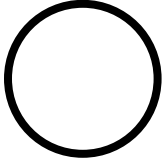
\includegraphics[scale=0.2]{Capitulo2/imagenes/Evento2} \\
		
		\hline
		{\small Temporizador } & {\small El disparador son una fecha y hora específicos, o un intervalo de tiempo regular (por ejemplo, el primer viernes de cada mes a las 8am). } & \vspace{2mm} \hspace{2mm} 
\includegraphics[scale=0.2]{Capitulo2/imagenes/EventoT}\\
		
		\hline
		{\small Mensaje } & {\small El disparador es un mensaje que llega desde otra entidad de negocio o rol (participante). Por ejemplo, un cliente pide una verificación de su cuenta. } & \vspace{1mm} \hspace{2mm} 
\includegraphics[scale=0.2]{Capitulo2/imagenes/EventoM}\\
		
		\hline		
		{\small Señal } & {\small  El disparador es una señal difundida desde otro proceso. Por ejemplo, un proceso difunde un cambio en la tasa de interés, disparando cierta cantidad de procesos a iniciarse como resultado.}  &  \vspace{1mm} \hspace{2mm} 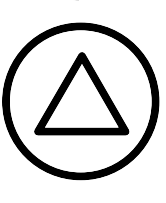
\includegraphics[scale=0.2]{Capitulo2/imagenes/EventoS}\\ 
		
		\hline
		{\small Condicional } & {\small El disparador es una expresión de condición que debe ser satisfecha para que empiece el proceso. } & \vspace{1mm} \hspace{2mm} \includegraphics[scale=0.2]{Capitulo2/imagenes/Eventoc}\\
		
		\hline
		{\small Múltiple } & {\small Define uno o más disparadores que puede ser cualquier combinación de mensajes, temporizadores, condiciones o señales (cualquiera de los cuales inicia un proceso). } & \vspace{1mm} \hspace{2mm} 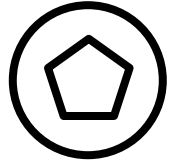
\includegraphics[scale=0.2]{Capitulo2/imagenes/EventoMul}\\
		\hline
		\end{tabular}    
		\caption{Eventos de inicio \citep{stephena2009}}
		\label{tabla:Eventosdeinicio}
\end{table}

\subsubsection{Eventos intermedios}
Un evento intermedio es algo que ocurre durante la ejecución de un proceso, estos eventos afectan el flujo del prceso.

\begin{table}[H]
	\centering
	\begin{tabular}{ |p{2cm}|p{9.5cm}|p{1.7cm}|p{1.7cm}|  }
		\hline
		\multicolumn{4}{|c|}{Eventos intermedios} \\
		\hline
		\textbf{Elemento}& \textbf{Descripción}&\textbf{Envío} & \textbf{Recepción}\\
		
		\hline
		{\small Básico } & {\small No se define ningún disparador.  } & &\vspace{0.5mm} \hspace{2mm} 
\includegraphics[scale=0.2]{Capitulo2/imagenes/BasicoR} \\
		
		\hline
		{\small Temporizador } & {\small El disparador son una fecha y hora específicos, o un intervalo de tiempo regular (por ejemplo, el primer viernes de cada mes a las 8am). } & &\vspace{0.5mm} \hspace{2mm} 
\includegraphics[scale=0.2]{Capitulo2/imagenes/TemporizadorR} \\

		
		\hline
		{\small Mensaje } & {\small El disparador es un mensaje. El mensaje debe ser enviado a otra entidad de negocio en el proceso, o debe ser recibido de una de estas. Estas entidades de negocio (participantes), si se muestran en el diagrama, son representadas por Pools(Participantes). } & \vspace{0.5mm} \hspace{2mm} 
\includegraphics[scale=0.2]{Capitulo2/imagenes/MensajeE} &\vspace{0.5mm} \hspace{2mm} 
\includegraphics[scale=0.2]{Capitulo2/imagenes/MensajeR} \\
		\hline
		
		\hline
		{\small Señal } & {\small El diagrama es una señal que se emite o recibe. } & \vspace{0.5mm} \hspace{2mm} \includegraphics[scale=0.2]{Capitulo2/imagenes/SeñalE} &\vspace{0.5mm} \hspace{2mm} \includegraphics[scale=0.2]{Capitulo2/imagenes/SeñalR} \\

		
		\hline
		{\small Error } & {\small Define un evento que normalmente interrumpirá el Proceso o requerirá corrección. } & &\vspace{0.5mm} \hspace{2mm} 
\includegraphics[scale=0.2]{Capitulo2/imagenes/Error} \\
		\hline
		
		\hline
		{\small Vínculo } & {\small Es utilizado para crear un mecanismo visual ``Go To'', ocultando un flujo de secuencia largo, o para establecer conectores ``off-page'', para imprimir. } & \vspace{0.5mm} \hspace{2mm} 
\includegraphics[scale=0.2]{Capitulo2/imagenes/VinculoR} &\vspace{0.5mm} \hspace{2mm} 
\includegraphics[scale=0.2]{Capitulo2/imagenes/VinculoE} \\
		\hline
	\end{tabular}    
	\caption{Eventos intermedios \citep{stephena2009}}
	\label{tabla:Eventosintermedio}
\end{table}

\subsubsection{Eventos finales}
Un evento final marca cuando un proceso, o más especificamente un ``camino'' dentro de un proceso, finaliza nn evento final es un pequeño círculo abierto con una única línea gruesa marcando su límite.

\begin{table}[H]
	\centering
	\begin{tabular}{ |p{2cm}|p{9.5cm}|p{1.7cm} |  }
		\hline
		\multicolumn{3}{|c|}{Eventos finiales} \\
		\hline
		\textbf{Elemento}& \textbf{Descripción}&\textbf{Notación}\\
		
		\hline
		{\small Simple } & {\small No se define ningún resultado. } & \vspace{0.5mm} \hspace{2mm} 
\includegraphics[scale=0.2]{Capitulo2/imagenes/BasicoF} \\
		
		\hline
		{\small Mensaje } & {\small Comunicación con otra entidad de negocio (participante o proceso). } & \vspace{2mm} \hspace{2mm} 
\includegraphics[scale=0.2]{Capitulo2/imagenes/MensajeF}\\
		
		\hline
		{\small Señal } & {\small El diagrama es una señal que se emite o recibe.. } & \vspace{1mm} \hspace{2mm} \includegraphics[scale=0.2]{Capitulo2/imagenes/SeñarT}\\
		
		\hline		
		{\small Error } & {\small  Un estado final que interrumpirá el proceso de transacción.}  &  \vspace{1mm} \hspace{2mm} 
\includegraphics[scale=0.2]{Capitulo2/imagenes/ErrorF}\\ 
		
		\hline
		{\small Compensación } & {\small Usado además como parte del comportamiento del sub-proceso de transacción, este evento lanza el disparador para deshacer (en caso que la instancia necesite ser deshechada). Puede estar vinculado a una actividad específica, o puede dejarse como un evento general de compensación, caso en el cual se aplica globalmente a esta instancia. } & \vspace{1mm} \hspace{2mm} 
\includegraphics[scale=0.2]{Capitulo2/imagenes/CompensacionF}\\
		
		\hline
		{\small Terminador } & {\small Detiene todas las actividades del proceso, incluso si están en curso otros hilos de ejecución. } & \vspace{1mm} \hspace{2mm} 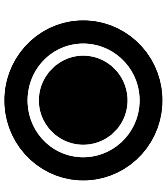
\includegraphics[scale=0.2]{Capitulo2/imagenes/EventoTer}\\
		\hline
	\end{tabular}    
	\caption{Eventos de inicio \citep{stephena2009}}
	\label{tabla:Eventosdeinicio}
\end{table}

\subsection{Gateway}
Las compuertas o gateways en BPMN son puntos de decisión que pueden ajustar la ruta de un flujo según ciertas condiciones.
\begin{table}[H]
	\centering
	\begin{tabular}{|p{2cm}|p{9.5cm}|p{1.7cm} |}
		\hline
		\multicolumn{3}{|c|}{Tipos de gateways} \\
		\hline
		\textbf{Elemento}& \textbf{Descripción}&\textbf{Notación}\\
		\hline
		{\small Exclusiva } & {\small En un punto de bifurcación, selecciona exactamente un flujo de secuencia de entre las alternativas existentes. En un punto de convergencia, la compuerta espera a que un flujo incidente complete para activar el flujo saliente.} & \vspace{0.5mm} \hspace{2mm} 
\includegraphics[scale=0.1]{Capitulo2/imagenes/gatewayE} \\
		
		\hline
		{\small Basada en eventos } & {\small Esta compuerta siempre será seguida por eventos o tareas de recepción, y sólo activará un flujo saliente dependiendo del evento que ocurra en primer lugar.} & \vspace{0.5mm} \hspace{2mm} 
\includegraphics[scale=0.1]{Capitulo2/imagenes/gatewayBE} \\
		
		\hline
		{\small Paralela } & {\small En un punto de bifurcación, todos los caminos salientes serán activados simultáneamente. En un punto de convergencia, la compuerta espera a que todos los flujos incidentes completen antes de activar el flujo saliente.} & \vspace{0.5mm} \hspace{2mm} 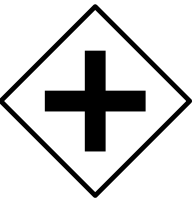
\includegraphics[scale=0.1]{Capitulo2/imagenes/gatewayP} \\
		\hline
		
		{\small Inclusiva } & {\small En un punto de bifurcación, al menos un flujo es activado. En un punto de convergencia, espera a todos los flujos que fueron activados para activar al saliente.} & \vspace{0.5mm} \hspace{2mm} 
\includegraphics[scale=0.1]{Capitulo2/imagenes/gatewayI} \\
		\hline

		{\small Compleja } & {\small Comportamiento complejo de convergencia/bifurcación no capturado por el resto de compuertas.} & \vspace{0.5mm} \hspace{2mm} 
\includegraphics[scale=0.1]{Capitulo2/imagenes/gatewayC} \\

		
		\hline
		{\small Exclusiva basada en eventos } & {\small En la ocurrencia de uno de los eventos subsecuentes se crea una nueva instancia del proceso.} & \vspace{0.5mm} \hspace{2mm} 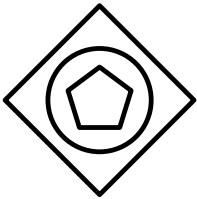
\includegraphics[scale=0.1]{Capitulo2/imagenes/gatewayEBE} \\
		\hline
		

		{\small Paralela basada en eventos  } & {\small En la ocurrencia de uno de los eventos subsecuentes se crea una nueva instancia del proceso.} & \vspace{0.5mm} \hspace{2.5mm} 
\includegraphics[scale=0.1]{Capitulo2/imagenes/gatewayPBE} \\
		\hline
	\end{tabular}
		\caption{Tipos degateways}
\label{tabla:Tiposdegateways}
\end{table}

\subsection{Actividad}
Una actividad se representa mediante un rectángulo de esquinas redondeadas (Figura ~\ref{fig:Actividad}) y es un término genérico para trabajos que la empresa realiza. Una actividad puede ser atómica o no atómica (compuesta).
Las actividades representan acciones, por tanto, una acción es una actividad. Existen dos tipos, actividades atómicas/simples y actividades compuestas/subprocesos. Las actividades atómicas/simples son aquellas que ya no se pueden desagregar en otras y se utilizan para elaborar diagramas a su nivel más bajo de detalle.\\
Las actividades son la espina dorsal de los procesos, debido a que son las actividades las que transforman el estado de un objeto de negocio para que el proceso puede llegar a producir valor para los clientes. Las actividades se pueden definir como acción sobre un objeto, es decir, una actividad se denomina siempre con un verbo (acción) y un sustantivo(objeto). Por ejemplo ``Revisar solicitud'' \citep{hitpass2017bpm}.
\newline
Los tipos de actividades son: 
\begin{figure}[h]
	\centering
	
\includegraphics[scale=0.2]{Capitulo2/imagenes/Actividad} 
	\caption{Actividad}
	\label{fig:Actividad}
\end{figure}

 Los tipos de actividades son: 

\begin{itemize}
	\item \textbf{Tarea:} Una tarea es una unidad de trabajo, el trabajo a realizar. Cuando aparece con el símbolo (+) indica un subproceso, una actividad que puede ser refinada como se ve en la figura ~\ref{fig:Tarea}.
	\begin{figure}[H]
		\centering
		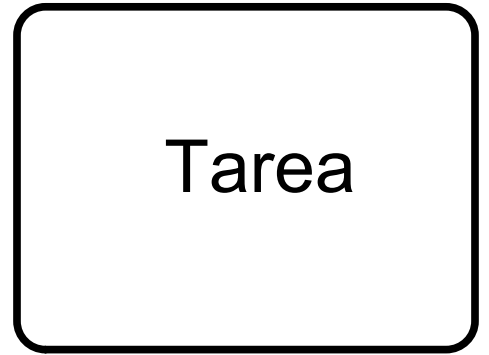
\includegraphics[scale=0.2]{Capitulo2/imagenes/tarea} 
		\caption{Tarea}
		\label{fig:Tarea}
	\end{figure}
	
	\item \textbf{Transacción:} Una Transacción es un conjunto de actividades relacionadas lógicamente, adhiriéndose a un protocolo transaccional particular como se ve en la figura ~\ref{fig:Transaccion}.
	\begin{figure}[h]
		\centering
		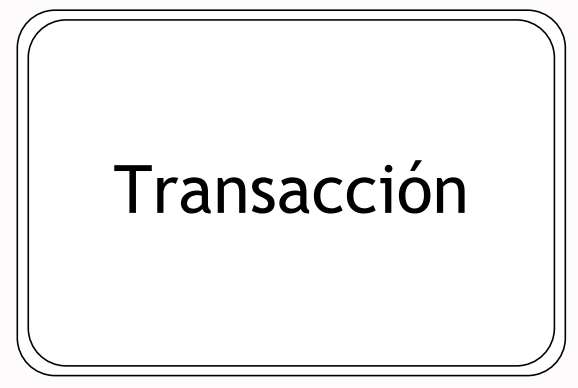
\includegraphics[scale=0.2]{Capitulo2/imagenes/Transaccion} 
		\caption{Transaccion}
		\label{fig:Transaccion}
	\end{figure}
	
	
	\item \textbf{Subproceso de evento:} Un subproceso (figura ~\ref{fig:SubPEvento}) de evento se situa en el interior de otro (sub)proceso. Este se activa en la ocurrencia del evento de inicio especificado y mientras el proceso que lo contiene permanezca también activo. El subproceso de evento puede interrumpir o no al proceso que lo contiene.
	
	\begin{figure}[h]
		\centering
		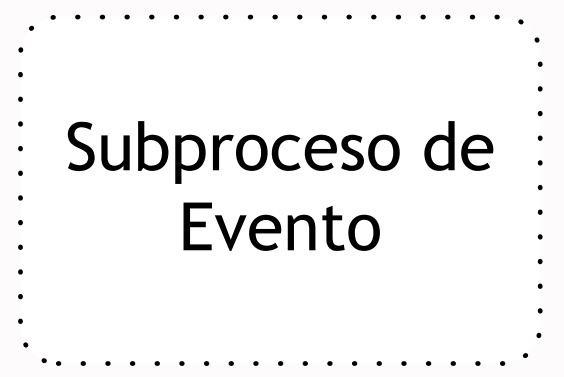
\includegraphics[scale=0.2]{Capitulo2/imagenes/SubPEvento} 
		\caption{Subproceso de evento}
		\label{fig:SubPEvento}
	\end{figure}
	\item \textbf{Actividad de llamada:} Una actividad de llamada es una referencia a un subproceso o tarea definido de forma global que se reutiliza en el proceso actual figura ~\ref{fig:SubPEvento2}.
	\begin{figure}[h]
		\centering
		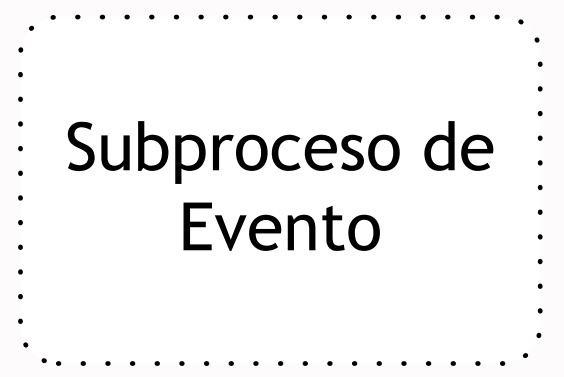
\includegraphics[scale=0.2]{Capitulo2/imagenes/SubPEvento} 
		\caption{Subproceso de evento}
		\label{fig:SubPEvento2}
	\end{figure}
\end{itemize}

\subsubsection{Tarea}
Las tareas son actividades atómicas utilizadas cuando el trabajo que se esta realizando no se puede descomponer a un nivel más detallado. Las tareas son llevadas a cabo por una persona y/o por una aplicación.

\begin{table}[H]
	\centering
	\begin{tabular}{|p{2cm}|p{9.5cm}|p{1.7cm} |}
	\hline
	\multicolumn{3}{|c|}{Tipos de tareas} \\
	\hline
	\textbf{Elemento}& \textbf{Descripción}&\textbf{Notación}\\
	\hline
	{\small Usuario } & {\small Representa el trabajo realizado por un usuario de un sistema conectado al motor de flujo de trabajo. Ejemplo: Registrar un empleado.} & \vspace{0.5mm} \hspace{2mm} 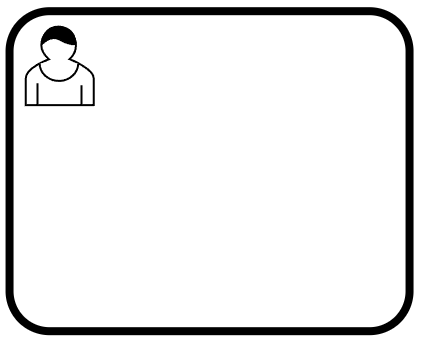
\includegraphics[scale=0.1]{Capitulo2/imagenes/TUsuario} \\
	
	\hline
	{\small Manual } & {\small Representa una tarea realizada por una persona que no utiliza un sistema de workflow. Ejemplo: Servir café.} & \vspace{0.5mm} \hspace{2mm} 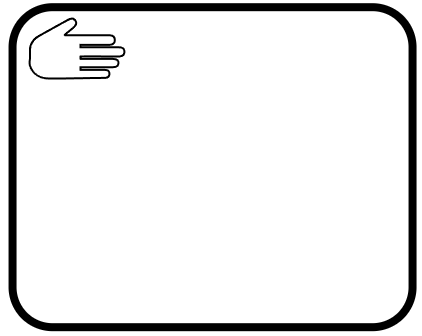
\includegraphics[scale=0.1]{Capitulo2/imagenes/TManual} \\
	
	\hline
	{\small Envío de mensajes } & {\small Envía un mensaje a otro proceso y avanza automáticamente a la siguiente tarea, que normalmente es una tarea de recepción o un evento intermedio de captura de mensajes.} & \vspace{0.5mm} \hspace{2mm} 
\includegraphics[scale=0.1]{Capitulo2/imagenes/TEMensaje} \\
	\hline
	
	{\small Recepción de mensajes } & {\small Espera la recepción de un mensaje desde otro proceso. Normalmente se coloca después de una tarea de envío de mensajes o un evento intermedio de lanzamiento de mensajes.} & \vspace{0.5mm} \hspace{2mm} 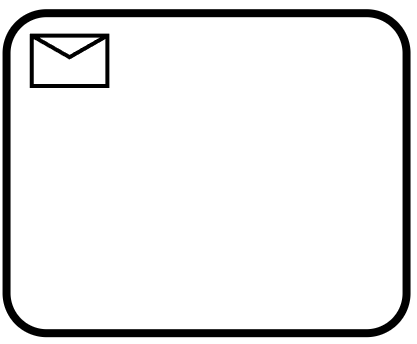
\includegraphics[scale=0.1]{Capitulo2/imagenes/TRMensaje} \\
		
	\hline
	{\small Servicio } & {\small Ejecuta un servicio web y se utiliza para implementar integraciones con sistemas de información.} & \vspace{0.5mm} \hspace{2mm} 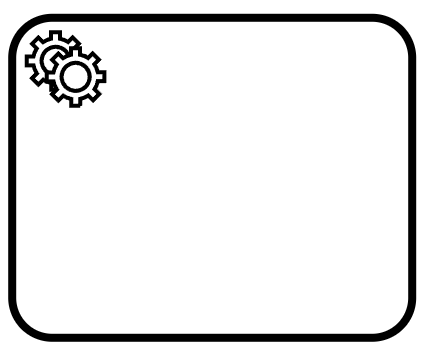
\includegraphics[scale=0.1]{Capitulo2/imagenes/TServicio} \\
		
	\hline
	{\small Regla de negocio } & {\small Acciona una regla de negocio que devuelve un valor para la comparación. Se puede realizar a través de una llamada de servicio web.} & \vspace{0.5mm} \hspace{2mm} 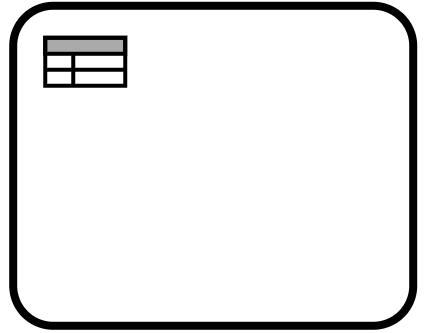
\includegraphics[scale=0.1]{Capitulo2/imagenes/TRNegocio} \\
		\hline
		
	{\small Script } & {\small Ejecuta una secuencia de comandos utilizando el propio motor de procesos. Se puede utilizar, por ejemplo, para ejecutar una secuencia de comandos de Powershell.} & \vspace{0.5mm} \hspace{2mm} 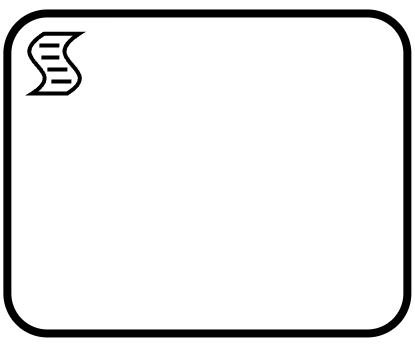
\includegraphics[scale=0.1]{Capitulo2/imagenes/TScript} \\
		\hline
		
		
	\end{tabular}
	\caption{Tipos de tareas \citep{Bauab2018}}
	\label{tabla:tiposDeTareas}
\end{table}

\subsubsection{Subprocesos}
Un subproceso es un conjunto de actividades incluidas dentro de un
proceso. Puede desglosarse en diferentes niveles de detalle denominadas
tareas. Se representa con un símbolo de suma en la parte central inferior
de la figura. A continuación se presentan los tipos de subprocesos:

\begin{itemize}
	\item \textbf{Colapsada: }Esta versión de Subproceso se ve como una tarea con la adición de un signo más en la parte central inferior (Figura ~\ref{subprocesoC}. Los detalles del sub-proceso no son visibles en el diagrama.
	
	\begin{figure}[H]
		\centering
		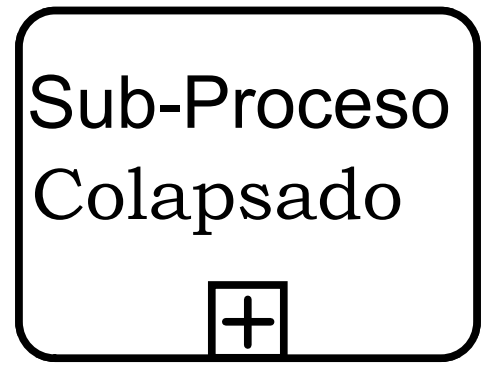
\includegraphics[scale=0.2]{Capitulo2/imagenes/subprocesoC} 
		\caption{Sub-proceso colapsado}
		\label{subprocesoC}
	\end{figure}
	\item \textbf{Expandida: }Esta versión de forma del Sub-proceso es ``estirada'' y abierta para que los detalles de sub-proceso sean visibles dentro de los límites de la forma. en este caso no hay ningún marcador en la parte inferior central de la forma. Sin embargo, algunas herramientas de modelado de procesos colocan un pequeño signo de menos (-) en la parte inferior central de la forma para indicar que el sub-proceso  puede ser colapsado.
\end{itemize}

\subsection{Swimlanes}
Swimlanes ayuda a partir y ordenar las actividades en un diagrama. Hay dos tipos: Pools y Carriles.
\subsubsection{Pool o participantes}
Un Pool es la representación gráfica de un Participante en una Colaboración. Un participante (Figura ~\ref{Pool}) puede ser un PartnerEntity específico (por ejemplo, una empresa) o puede ser un PartnerRole más general (por ejemplo, un comprador, vendedor o fabricante). Un Pool puede o no puede hacer referencia a un proceso. No se requiere que un pool contenga un proceso, es decir, puede ser una “caja negra” \citep{VonRosing2014}.
\begin{figure}[H]
	\centering
	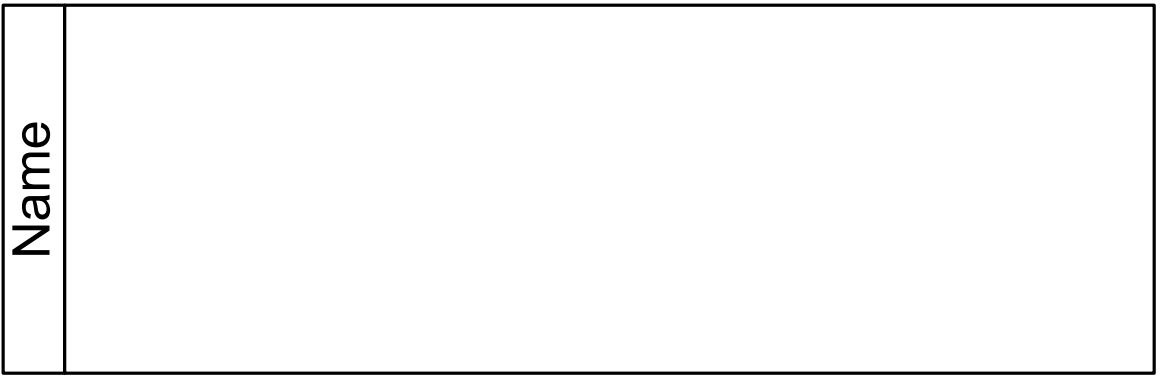
\includegraphics[scale=0.2]{Capitulo2/imagenes/Pool}
	\caption{Pool o participante}
	\label{Pool}
\end{figure}

\subsubsection{Carriles}
Utilizados a menudo para representar roles de negocio internos dentro de un proceso, los carriles en realidad proveen un mecanismo genérico para particionar los objetos dentro de un pool o participante, basado en las características del proceso o elementos \citep{stephena2009}.
\begin{figure}[H]
	\centering
	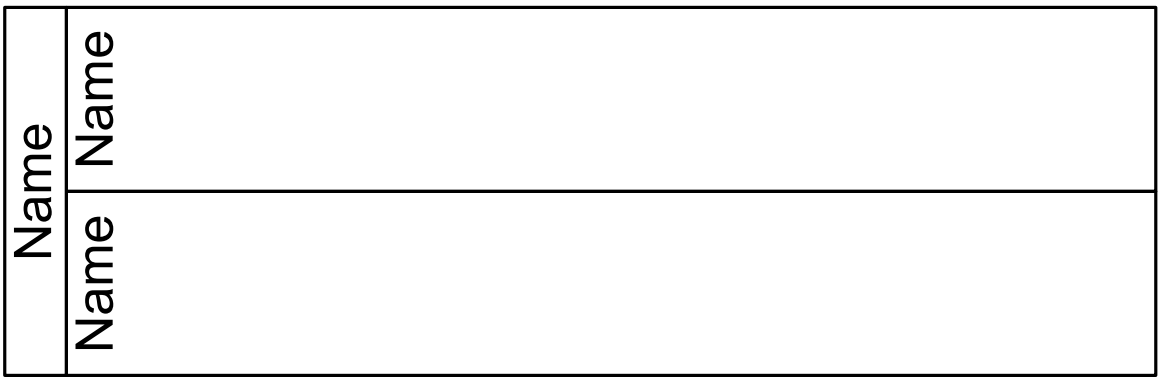
\includegraphics[scale=0.2]{Capitulo2/imagenes/Carril}
	\caption{Carril}
	\label{Carril}
\end{figure}

\subsection{Conectores}
Los conectores vinculan dos objetos en un diagrama. Existen tres diferentes tipos de conectores.

\begin{itemize}
	\item \textbf{Flujo de secuencia: }Define el orden adecuado y conecta los objetos de flujo.
	\begin{figure}[H]
		\centering
		\includegraphics[scale=0.2]{Capitulo2/imagenes/FlujoDeSecuencia.png}
		\caption{Flujo de secuencia}
		\label{FSecuencia}
	\end{figure}
	\item \textbf{Flujo de mensaje: }Define el flujo de mensajes de un participante de un proceso a otro.
	\begin{figure}[H]
		\centering
		\includegraphics[scale=0.2]{Capitulo2/imagenes/FlujoDeMensaje.png}
		\caption{Flujo de mensaje}
		\label{FMensaje}
	\end{figure}
	\item \textbf{Asociaciones: }Define las relaciones entre los artefactos y objetos del flujo.
	\begin{figure}[H]
		\centering
		\includegraphics[scale=0.2]{Capitulo2/imagenes/Asociacion.png}
		\caption{Asociación}
		\label{Asociación}
	\end{figure}
\end{itemize}
\subsection{Artefactos}
Los artefactos proporcionan un mecanismo para capturar información adicional sobre un proceso, más allá de la estructura subyacente de los diagramas de flujo. Esta información no afecta directamente las características del diagrama de flujo de un proceso.

\begin{itemize}
	\item \textbf{Objetos de datos: }Se utiliza para representar los documentos y datos que son manipulados por los procesos. Son como representantes de la ""Carga útil"" del proceso \citep{stephena2009}.
	\begin{figure}[H]
		\centering
		\includegraphics[scale=0.3]{Capitulo2/imagenes/ObjetoDeDato.png}
		\caption{Objetos de datos}
		\label{Odatos}
	\end{figure}
	
	\item \textbf{Grupos: }Proporciona un mecanismo para resaltar y clasificar una sección del modelo o conjunto de Objetos. \citep{stephena2009}.
	\begin{figure}[H]
		\centering
		\includegraphics[scale=0.3]{Capitulo2/imagenes/Grupo.png}
		\caption{Grupos}
		\label{Grupos}
	\end{figure}
	
	\item \textbf{Anotaciones de texto: }Añaden más información descriptiva a un modelo.
	\begin{figure}[H]
		\centering
		\includegraphics[scale=0.3]{Capitulo2/imagenes/Anotacion.png}
		\caption{Anotacion de texto}
		\label{Atexto}
	\end{figure}
	
\end{itemize} 

\section{Herramientas}
\subsection{Power Automate}
Power Automate es una herramienta de flujo de trabajo que permite la automatización de procesos al estilo
evento-a-acción dentro y fuera del conjunto de tecnologías de Microsoft 365. Ofrece conectores externos y la capacidad de
construir conectores externos personalizados hacia y desde otras tecnologías \citet{Critchley2020}.

Power Automate es un servicio de flujo de trabajo en línea que automatiza acciones en las aplicaciones y servicios más comunes. Por ejemplo, puede crear un flujo que agregue un cliente potencial a Microsoft Dynamics 365 y un registro en MailChimp cada vez que alguien con más de 100 seguidores tuitee sobre una empresa.

Cuando se registra, puede conectarse a más de 500 servicios y puede administrar datos en la nube o en fuentes locales como SharePoint y Microsoft SQL Server. La lista de aplicaciones que puede usar con Power Automate crece constantemente \citep{MicrosoftLearn}.

Cuenta con los siguientes tipos de flujos de nube.

\begin{itemize}
	\item \textbf{Flujos automatizados:}	Crear una automatización que se desencadena por un evento como la llegada de un correo electrónico de una persona específica o una mención de la empresa en las redes sociales.
	\item \textbf{Flujos instantáneos:}	Iniciar una automatización con un clic de un botón. Puede automatizar las tareas repetitivas desde el escritorio o dispositivos móviles. Por ejemplo, envíe instantáneamente un recordatorio al equipo con solo presionar un botón desde el dispositivo móvil.
	\item \textbf{Flujos programados:}	Programar una automatización como la carga diaria de datos a SharePoint o una base de datos.
\end{itemize}

\subsection{Power Apps}
Power apps permite a las organizaciones crear e implementar aplicaciones personalizadas que optimizan los
procesos comerciales y mejorar la productividad. Además, Power apps permite a los usuarios crear aplicaciones sin escribir
código, lo que hace posible que los empleados no técnicos obtengan tanto valor de la plataforma como el personal técnico \citep{Pearson2020}.
\subsubsection{Power Apps Studio}
Power Apps Studio es el diseñador de aplicaciones que se usa para compilar aplicaciones de lienzo. El diseñador de aplicaciones hace que la creación de estas se parezca más a la creación de un conjunto de diapositivas en Microsoft PowerPoint \citep{Microsoft}.

\subsection{Power BI}
En pocas palabras, Power BI permite a las organizaciones convertir los datos brutos en información útil que impulsa
una visión empresarial más profunda e informa la toma de decisiones \citet{Pearson2020}.
\subsection{Sharepoint}
Las organizaciones usan Microsoft SharePoint para crear sitios web. Se puede usar como un lugar seguro donde
almacenar, organizar y compartir información desde cualquier dispositivo, así como acceder a ella. Lo que se necesita es un
explorador web, como Microsoft Edge, Internet Explorer, Chrome o Firefox \citet{Microsoft}.

\subsubsection{Listas de Shapoint}
Una lista es una colección de datos que puede compartir con los miembros del equipo y con las personas a las que ha proporcionado acceso. Hay una serie de plantillas de listas base para usar como punto de partida para organizar elementos de lista \citep{Microsoft}.

Las listas de Sharepoint se pueden usar como una base de persistencia de datos o base de datos en dichas listas se puede crear columnas como:

\begin{itemize}
	\item \textbf{Una sola línea de texto: }En este tipo de columnas podemos almacenar cadenas de texto con un límite de hasta 255 caracteres.
	\item \textbf{Varias lineas de texto: }En este tipo de columna podemos almacenar cadenas de texto con más de de 255 carácteres.
	\item \textbf{Número: }En este tipo de columna se puede almacenar datos de tipo numérico no distingue de decimales o enteros, agrupa todos eso tipos de datos en una sola.
	\item \textbf{Sí/No: }En este tipo de columna se puede almacenar valores de sí o no o true o false parecidos a los datos booleanos que se manejan en distintos lenguajes de programación.
	\item \textbf{Usuario: }Este tipo de columna almacena objetos complejos de tipo User, se almacena en un campo datos como el nombre, correo, foto, etc.
	\item \textbf{Fecha y Hora: } En este tipo de columna se puede almacenar valores de tipo fecha parecido a los campos Date que se manejan en distintos lengujes de programación.
	\item \textbf{Opción: }En este tipo de columna se puede almacenar un objeto de valores permitidos, pueden ser varios elemento o solo uno depende del tipo de configuración que se le de.
\end{itemize}

\subsection{Microsoft Forms}
Microsoft Forms es una herramienta para la recolección de datos ya sea por medio de encuestas o
cuestionarios para su posterior manipulación.
\subsection{Power Virtual Agents}
Crea fácilmente chatbots para conversar con los clientes y empleados sin necesidad de escribir
código \citet{Pearson2020}.           % ~20 páginas - Poner un contexto a la tesis, hacer referencia a trabajos actuales en el tema
	\chapter{Automatización de cajeros automáticos}
En este capítulo, se analizó y modeló un proceso asignado por un colaborador del banco de Bogotá, el modelado del proceso se hizo usando el estándar BPMN definido en el capítulo ~\ref{ch:BPMN}.

\section{Descripción del proceso (Automatización de cajeros automáticos)}
Desde un área de Canales Electrónicos del banco de Bogotá surgió una iniciativa para automatizar el proceso de informar sobre el estado de los cajeros automáticos del Banco de Bogotá, donde cualquier colaborador puede reportar las fallas que encuentre en los cajeros automáticos usando un formulario que activa un flujo de Power Automate que requiere el código o la dirección específica del cajero en cuestión. Cuando un colaborador del banco encuentra un cajero con una falla, este tiene la posibilidad de informar al área encargada de esta falla, dependiendo de la región la falla se le notifica a una persona en específico para que gestione y repare la falla del cajero.

Modelo resultante (figura ~\ref{fig:AcA}).

\begin{figure}[H]
	\centering
	\includegraphics[scale=0.25]{Capitulo3/imagenes/diagram-Cajeros.png}
	\caption{Automatización de cajeros automáticos}
	\label{fig:AcA}
\end{figure}

\section{Construcción del modelo}

\subsection{Participantes}
Dentro de la descripción se pudieron identificar los siguientes participantes: 
\begin{itemize}
	\item \textbf{Colaborador: }Es el colaborador que inicia el flujo al  solicitar mantenimiento del cajero automático.
	\item \textbf{Analista: } Es la persona encargada de darle solución al caso.
	\item \textbf{Mantenimiento: } Es un participante del proceso que interfiere directamente en el proceso al hacerle mantenimiento a los cajeros.
\end{itemize}

Ya con los participantes identificados se da inicio al proceso usando un evento de inicio básico, cuando el colaborador está haciendo la solicitud tiene la opción de notificar la falla del cajero e identificarlo por la dirección en la cual está ubicado el cajero o por un código único que los identifica.

\begin{figure}[H]
	\centering
	\includegraphics[scale=0.5]{Capitulo3/imagenes/1.png}
	\caption{¿Cuenta con el código del cajero?}
	\label{CodCaj}
\end{figure}

El proceso debe consultar a que analista le corresponde el cajero (Por zona se tiene un analista asignado), se consulta en la base de datos el analista al que se debe notificar, también se le notifica al colaborador que su solicitud fue recibida y este está enterado.

\begin{figure}[H]
	\centering
	\includegraphics[scale=0.5]{Capitulo3/imagenes/2.png}
	\caption{¿Cuenta con el código del cajero?}
	\label{CodCaj2}
\end{figure}

Cuando el analista recibe la notificación debe hacer la gestión con el participante encargado del mantenimiento, el analista debe hacer la solicitud a mantenimiento y esperar que este le notifique que el mantenimiento está completo.

\begin{figure}[H]
	\centering
	\includegraphics[scale=0.5]{Capitulo3/imagenes/3.png}
	\caption{Notificaciones}
	\label{notificaciones}
\end{figure}

Seguido se notifica al colaborador que se le dio solución al caso y se cierra el proceso.
\begin{figure}[H]
	\centering
	\includegraphics[scale=0.5]{Capitulo3/imagenes/4.png}
	\caption{Final del proceso}
	\label{Finproceso}
\end{figure}

\section{Implementación}
\subsection{Lista en SharePoint}\label{listasSp}
La lista de SharePoint es la herramienta que se usa dentro de la organización para coleccionar y organizar datos que se usan o consumen los flujos de Power Automate, la estructura de la lista así como los tipos de columna se hicieron acorde a la solicitud del colaborador de Canales electrónicos
.
\subsubsection{Lista Novedades en ATM}
\begin{figure}[H]
	\centering
	\includegraphics[scale=0.37]{Capitulo3/imagenes/6.png}
	\caption{Oficinas Novedades en ATM}
	\label{ListaNovedadesEnATM}
\end{figure}

\subsubsection{Lista Novedades en ATM}
\begin{figure}[H]
	\centering
	\includegraphics[scale=0.37]{Capitulo3/imagenes/7.png}
	\caption{Oficinas Novedades en ATM}
	\label{ListaNovedadesEnATM2}
\end{figure}

Las columnas se configuraron de la siguiente manera.

\begin{itemize}
	\item \textbf{ID: }Es una columna numérica única autoincrementable que define SharePoint de manera automática.
	\item \textbf{Fecha: } Esta columna toma valores dependiendo de la fecha de cierre del caso, esta columna se configuró como ``Fecha''.
	\item \textbf{Tiene código cajero: }Esta columna almacenará valores de tipo booleano (true o false), dependiendo si tiene o no el código de cajero a reportar.
	\item \textbf{Código cajero: }Es una columna numérica que almacena los códigos de los cajeros, es un número de cuatro dígitos, esta columna se definió de tipo ``Número''.
	\item \textbf{Dirección: } Es un valor alfabético o alfanumérico que define el nombre de una oficina, por este motivo se definió el tipo de la 
	columna como ``Una sola línea de texto''.
	\item \textbf{Falla: }Es un valor alfabético donde almacenamos la falla del cajero (Sin dinero, Falla en la lectura de la trajeta, etc), por este motivo definimos el tipo de la columna como ``Una sola línea de texto''.
	\item \textbf{Descripción: } Es un valor de tipo alfabético, pero debido a que el número de caracteres puede ser muy grande se define ``Varias líneas de texto'' debido a la capacidad que tienen de almacenar mayor cantidad de número de caracteres.
	\item \textbf{Analista: } Esta columna almacenará un objeto con los atributos (Nombre, Email, Cargo, etc.) del colaborador al cual se le asigne la solicitud, esta columna se configuró de tipo ``Usuario''.
	\item \textbf{Estados: }Esta columna almacena una serie de valores permitidos (Abierto, En trámite, Vencido, Cerrado, remitido erradamente, Atendido) pero solamente puede tomar uno de estos valores, esta columna se definió de tipo opción.
	\item \textbf{Respuesta: } Es un valor de tipo alfabético, pero debido a que el número de caracteres puede ser muy grande se define ``Varias líneas de texto'' debido a la capacidad que tienen de almacenar mayor cantidad de número de caracteres.
	\item \textbf{Ciudad: } Esta columna toma valores dependiendo de la ubicación del cajero, esta columna se configuró como ``Una sola línea de texto''.
	\item \textbf{Usuario solicitante: } Esta columna toma valores dependiendo de la ubicación del cajero, esta columna se configuró como ``Una sola línea de texto''.
	\item \textbf{Fecha de cierre: } Esta columna toma valores dependiendo de la fecha de cierre del caso, esta columna se configuró como ``Fecha''.
\end{itemize}

\subsubsection{Asignación analista}
\begin{figure}[H]
	\centering
	\includegraphics[scale=0.5]{Capitulo3/imagenes/8.png}
	\caption{Lista asignación analista}
	\label{Aanalista}
\end{figure}

\begin{itemize}
	\item \textbf{ID: }Es una columna numérica única autoincrementable  que define SharePoint de manera automática.
	\item \textbf{Analista: } En esta columna se almacenan valores de tipo alfanuméricos donde se guarda el nombre de distintos analistas y la ciudad o zona que tienen asignado, se definió de ``Una sola línea de texto''.
	\item \textbf{Ciudad: }Es un valor alfanumérico donde se almacena nombre de distintas ciudades o municipios, se definió de tipo ``Una sola línea de texto''.
\end{itemize}

\subsection{Forms}
En las figuras ~\ref{fig:FreporteFalla}, ~\ref{fig:CuentaCodigoDelCajero}, ~\ref{fig:CuentaCodigoDelCajero2} y ~\ref{fig:FinForm}. Se muestra el formulario donde los colaboradores del banco pueden reportar las falla de los cajeros automáticos.

\begin{figure}[H]
	\centering
	\includegraphics[scale=0.3]{Capitulo3/imagenes/f1.png}
	\caption{Formulario reporte falla cajero}
	\label{fig:FreporteFalla}
\end{figure}
\begin{figure}[H]
	\centering
	\includegraphics[scale=0.3]{Capitulo3/imagenes/f2.png}
	\caption{Cuenta con el código del cajero}
	\label{fig:CuentaCodigoDelCajero}
\end{figure}
\begin{figure}[H]
	\centering
	\includegraphics[scale=0.3]{Capitulo3/imagenes/f2.2.png}
	\caption{No cuenta con el código del cajero}
	\label{fig:CuentaCodigoDelCajero2}
\end{figure}
\begin{figure}[H]
	\centering
	\includegraphics[scale=0.3]{Capitulo3/imagenes/f3.png}
	\caption{Fin del formulario}
	\label{fig:FinForm}
\end{figure}

\subsection{Power Automate}
\subsubsection{Flujo Administración de cajeros automáticos}
Se definió un flujo de nube automatizado que se desencadena automáticamente al recibir una nueva respuesta del formulario ``Queremos tener siempre nuestros cajeros automáticos disponibles para ti'' ~\ref{fig:DesFlu}, seguido se ejecuta la acción ``Obtener los detalles de la respuesta''.
\begin{figure}[H]
	\centering
	\includegraphics[scale=0.5]{Capitulo3/imagenes/flujo1.png}
	\caption{Desencadenador del flujo}
	\label{fig:DesFlu}
\end{figure}

Las siguientes cuatro acciones ~\ref{fig:DeclVar} utilizan la acción ``Inicializar variable'', se declaran cuatro variables (VarCorreoAnalista, VarIDelemento, varFalla, VarVinculelemento) todas de tipo cadena estas, variables  que se usan en pasos posteriores.
\begin{figure}[H]
	\centering
	\includegraphics[scale=0.5]{Capitulo3/imagenes/flujo2.png}
	\caption{Declaración de variables}
	\label{fig:DeclVar}
\end{figure}

La siguiente acción ~\ref{fig:Consultaycondición} hace una consulta de la lista ``Asignación analista'' y trae aquellos campos que cumplan con la condición de la casilla consulta de filtro, en este caso se filtra por aquellos donde la Ciudad sea igual a la ciudad que respondieron en el formulario, luego una condición se divide el flujo en dos caminos con la respuesta de la pregunta ``¿Cuentas con el código del cajero automático?''.
\begin{figure}[H]
	\centering
	\includegraphics[scale=0.5]{Capitulo3/imagenes/flujo3.png}
	\caption{Consulta y condición}
	\label{fig:Consultaycondición}
\end{figure}

En caso de que el resultado de la condición sea verdadero, se establece la variable ``VarCorreoAnalista'' ~\ref{fig:Evar}, el cual se le asigna el ``Analista Email'' resultado de la salida de la acción ``Obtener elementos de Asignación analista (Lista)''. Se encierra en un ``aplicar a cada uno'' porque cuando se hace uso de la acción ``Obtener elemento'', una de las salidas es una lista de los elementos que coincidan con el filtro (Si se le define) y como es una lista Power Automate recorre la lista y aplica la o las acciones que contiene ``Aplicar a cada uno''.

\begin{figure}[H]
	\centering
	\includegraphics[scale=0.5]{Capitulo3/imagenes/flujo4.png}
	\caption{Establecer variable}
	\label{fig:Evar}
\end{figure}

El mismo caso con la acción ``Crear elemento 2'', dado que utiliza una salida (``Analista Claims'') de la acción ``Obtener elementos de Asignación analista (Lista)'' la acción se envuelve en un ``Aplicar a cada uno'' ~\ref{fig:CElemento}. La acción ``Crear elemento'' crea un nuevo elemento en la lista ``Noveades en ATM'' como parámetros de entrada, recibe la dirección del sitio de SharePoint donde se encuentra la lista y los elementos de la lista.

\begin{figure}[H]
	\centering
	\includegraphics[scale=0.5]{Capitulo3/imagenes/flujo5.png}
	\caption{Crear elemento}
	\label{fig:CElemento}
\end{figure}

Las siguientes acciones ~\ref{fig:EVariables} son de tipo ``Establecer variable'', esta acción  asigna el valor que se quiera dar a las variables.

\begin{figure}[H]
	\centering
	\includegraphics[scale=0.5]{Capitulo3/imagenes/flujo6.png}
	\caption{Establecer variables}
	\label{fig:EVariables}
\end{figure}

Con estas acciones acabaría el caso positivo de la condición ~\ref{fig:Cnegativo}. En el caso negativo, la primera acción que se define es una condición en la cual válida si insertaron un valor(adjunto) en la pregunta ``Si no cuentas con el código, carga aquí una imagen legible del cajero del Banco, donde podamos ver la placa frontal como lo muestra el ejemplo.'',  esta condición se hace con el fin de validar si respondieron la pregunta.

\begin{figure}[H]
	\centering
	\includegraphics[scale=0.5]{Capitulo3/imagenes/flujo7.png}
	\caption{Caso negativo}
	\label{fig:Cnegativo}
\end{figure}

En el caso positivo ~\ref{fig:Evar2} las acciones a ejecutar son ``Establecer variable'', el cual está encerrado dentro de un ``Aplicar a cada uno'' dado que usa las salidas de la acción ''Obtener elementos``.

\begin{figure}[H]
	\centering
	\includegraphics[scale=0.5]{Capitulo3/imagenes/flujo9.png}
	\caption{Establecer variable}
	\label{fig:Evar2}
\end{figure}

La siguiente acción `\ref{fig:Cele} es un ``crear elemento'' y dado que se usan salidas de la acción ``Obtener elementos'' se encierra dentro de un ``Aplicar a cada uno'' y se le pasan los parámetros correspondientes.

\begin{figure}[H]
	\centering
	\includegraphics[scale=0.5]{Capitulo3/imagenes/flujo10.png}
	\caption{Crear elemento}
	\label{fig:Cele}
\end{figure}

Cuando se adjunta un archivo a un formulario o encuesta, este guarda la información en la nube, y descompone el archivo en su contenido y nombre. La información la guarda en un JSON y se usa la acción ``Análisis del archivo JSON'' ~\ref{fig:Cele2}el cual recibe como entrada el archivo adjunto y devuelve los elementos del JSON. Donde ``driveId'' en conjunto con ``id'' forman un id único de cada archivo y por el cual el flujo lo puede identificar.
\\
La acción ``Obtener contenido de archivo'' es una acción que recibe como parámetro de entrada la identificación del archivo o la ruta donde este se encuentra ubicado, y como salida genera el archivo codificado en base64. La acción ``Agregar datos adjuntos'' Recibe como parámetros la dirección del sitio, el nombre de la lista, el identificador del elemento al que se quiere adjuntar los datos, un nombre que es una de las salidas que genera ``Análisis del archivo JSON'' y contenido del archivo que se le pasa de la salida que genera la acción ``Obtener contenido de archivo''.

\begin{figure}[H]
	\centering
	\includegraphics[scale=0.5]{Capitulo3/imagenes/flujo11.png}
	\caption{Adjuntar archivos en Sharepoint}
	\label{fig:Cele2}
\end{figure}

Las siguientes tres ~\ref{fig:defvar} acciones definen algunas variables que se inicializaron previamente, en este caso ``VarIDelemento'' variable en la que se almacena el id único que generan las listas de SharePoint, ``VarVinculoelemento'' se almacena un vínculo el cual lleva al elemento específico en la lista, ``VarFalla'' almacena la falla de la lista ``Novedades en ATM''.  Y con esto finaliza el caso positivo.

\begin{figure}[H]
	\centering
	\includegraphics[scale=0.5]{Capitulo3/imagenes/flujo12.png}
	\caption{Definición de variables}
	\label{fig:defvar}
\end{figure}

En el caso negativo solo se crea el elemento con la dirección que diligencie en el formulario.

\begin{figure}[H]
	\centering
	\includegraphics[scale=0.5]{Capitulo3/imagenes/flujo13.png}
	\caption{Crear elemento}
	\label{cele}
\end{figure}

Las siguientes cuatro ~\ref{fig:defvar2} acciones definen algunas variables que se habían inicializado previamente, en este caso ``VarIDelemento'' variable en la que se almacena el id único que generan las listas de SharePoint, ``VarVinculoelemento'' se almacena un vínculo el cual lleva al elemento específico en la lista, ``VarFalla'' almacena la falla de la lista ``Novedades en ATM'', ``VarCorreoAnalista'' donde se almacena el correo del analista encargado de dar solución al caso.

\begin{figure}[H]
	\centering
	\includegraphics[scale=0.5]{Capitulo3/imagenes/flujo14.png}
	\caption{Definición de variables}
	\label{fig:defvar2}
\end{figure}

Las siguientes dos acciones de Outlook son acciones las cuales reciben como parámetro a quien va dirigido el correo (usuario que envió el formulario en la primera y VarCorreoAnalista), el asunto en la primera acción se define como un texto fijo ``Solicitud creada ID: '' y dos variables ``VarIDelemento'' y ``VarFall'', en la segunda acción el texto fijo es ``Solicitud radicada ID: '' y complementan con el id del elemento (VarIDelemento) y la falla(VarFalla).
\\

El cuerpo en la primera acción es un texto fijo con el cual se notifica al colaborador que recibió la solicitud, y el cuerpo de la segunda acción notifica al analista que ha radicado una solicitud y se le envía la variable ``VarVinculoelemento''.

\begin{figure}[H]
	\centering
	\includegraphics[scale=0.5]{Capitulo3/imagenes/flujo15.png}
	\caption{Notificaciones}
	\label{not}
\end{figure}


\subsubsection{Notificación de respuesta}
Es un flujo ~\ref{fig:not2} más sencillo, ya que tiene como desencadenador ``Cuando se cree o modifica un elemento'' de la lista ``Novedades en ATM'', el flujo se desencadenará siempre que se cree o modifique en la lista, la acción siguiente es una condición en la que se verifica que el campo ``Respuesta'' de la lista ``Novedades en ATM'' no sea igual a ``Null'' o esté vacío y su estado sea igual a ``Atendido'', con solo una acción el caso positivo.
Cuando esa condición es cierta significa que el analista modificó el campo ``Respuesta'' y cambió el estado a ``Atendido''. Se envía un correo al usuario que hizo la solicitud notificándole que fue atendida, enviándole el ID de la solución y la ``Respuesta'' que haya dado el analista.

\begin{figure}[H]
	\centering
	\includegraphics[scale=0.5]{Capitulo3/imagenes/flujo16.png}
	\caption{Notificación usuario}
	\label{fig:not2}
\end{figure}
	\chapter{Automatización de canales BdB}
En este capítulo, se analizaró y modeló un proceso asignado por un colaborador del banco de Bogotá, el modelado del proceso se hará usando el estándar BPMN definido en el capítulo ~\ref{ch:BPMN}.


\section{Descripción del proceso (Automatización canales BdB)}
Desde área de Marketing y comunicaciones del banco de Bogotá surgió la iniciativa de automatizar el proceso de ``Canales'' donde las diferentes oficinas radican sus necesidades a las áreas de Publicidad y Mantenimiento, anteriormente las solicitudes que se le hacían al área de Marketing y comunicaciones se hacía por medio de correo electrónico y el seguimiento de estas se llevaba por medio de hojas de cálculo en Excel, la idea del área de marketing y comunicaciones es automatizar este proceso además de definir un canal por el cual las diferentes áreas puedan hacer sus solicitudes.\\

Para comenzar el proceso no lo puede iniciar cualquiera, el área de Marketing y comunicaciones recibe las solicitudes de los Jefes de oficinas, luego de que el Jefe de oficinas radique esta solicitud pasa a Client Partner Marketing el cual se encarga de validar las solicitudes que llegan al área, el tipo de solicitudes que llegan al área son las siguientes:\\
\begin{itemize}
	\item \textbf{Mantenimiento: } Los Jefes de oficina hacen estas solicitudes cuando  la pintura está dañada, una ventana rota, etc.
	\item \textbf{Otro: } Los Jefes de oficina seleccionan esta opción cuando piden una consulta (Referente a Marketing) o una recomendación.
	\item \textbf{Publicidad: }Los Jefes de oficina seleccionan esta opción cuando necesitan material publicitario como un afiche, tropezón, etc.
\end{itemize}

En caso de Mantenimiento Client Partner Marketing envía una notificación 
al Área administrativa y ellos se encargan del resto de la solicitud, cuando la solicitud es Otro, se le notifica al Comité de canales y ellos se encargan de gestionar la solicitud. En caso de Publicidad Client Partner Marketing asigna los estados de las solicitudes entrantes, entre las opciones que puede elegir están (Detenido, Cancelado y En progreso) donde cada estado define los siguientes pasos a ejecutar.
\begin{enumerate}
	\item Detenido: La solicitud se detiene y queda en este estado hasta que Cliente Partner Marketing le cambie el estado, una solicitud puede ser detenida por muchos factores, ejemplo la persona que hizo la solicitud se encuentra de vacaciones, etc.
	\item Cancelado: La solicitud se cancela y se le notifica al Jefe de oficinas que hizo la solicitud, las razones por la cuales se cancela la solicitud y se acaba el proceso.
	\item En progreso: La solicitud pasa de Client Partner Marketing a Client Partner Trade y se le notifica cuando esto sucede.
\end{enumerate}
En caso de la solicitud tener el estado de ``En progreso'' y haber notificado a Client Partner Trade, este gestiona y valida las solicitudes que le lleguen de Client Partner Markekting, también este puede cambiar el estado de las solicitudes entrantes puede elegir entre las opciones Detenido, Cancelado y En progreso, donde cada estado define los siguientes pasos a ejecutar:
\begin{enumerate}
	\item Detenido: La solicitud se detiene y queda en este estado hasta que Cliente Partner Trade le cambie el estado, una solicitud puede ser detenida por muchos factores, ejemplo la persona que hizo la solicitud se encuentra de vacaciones, etc.
	\item Cancelado: La solicitud se cancela y se le notifica a Client Partner Marketing porque se canceló y este a su vez al jefe de oficinas.
	\item En progreso: Se verifica si hay stock en bodega del material solicitado con Trade bodega.
\end{enumerate}

En caso de la solicitud tener el estado de ``En progreso'' y no tener stock en bodega, este le notifica a Client Partner Marketing y este a su vez al Jefe de oficinas y se cerraría el proceso.

En caso de haber stock se le envía una notificación al Jefe de oficinas con una fecha tentativa de entrega del material solicitado, también se le notifica a Client Partner Marketing que se va a realizar la entrega y también al analista de Trade, el analista de Trade debe alistar el material a enviar y notificar al proveedor de la entrega que se va a hacer, el proveedor le da una guía de seguimiento al analista de Trade y entrega el material a Client Partnert Marketing con un documento de entrega el Jefe de oficinas debe confirmar que recibió el material y notificar a Trade bodega para que este haga el cargue de documento de entrega y cerrar el proceso.\\

Modelo resultante (figura ~\ref{ABdB}).

\begin{figure}
	\centering
	\includegraphics[scale=0.2]{Capitulo4/imagenes/diagram.png}
	\caption{Automatización de canales BdB }
	\label{ABdB}
\end{figure}

\section{Construcción del modelo}

\subsection{Participantes}
Dentro de la descripción podemos obtener los siguientes participantes: 
\begin{itemize}
	\item \textbf{Jefe de oficinas: }Es el colaborador que inicia el flujo al hacer la solicitud de publicidad, mantenimiento u otro.
	\item \textbf{Client Partner Marketing: } Colaborador de área de Marketing y comunicaciones que se encarga de gestionar todas las solicitudes entrantes.
	\item \textbf{Comite de canales: } Comité que al que se redirigen las solicitudes cuando es de tipo Otro, este participante es una ``Caja negra'' debido a que interactúa con el proceso, pero no hace parte del proceso.
	\item \textbf{Área administrativa: }Área a la que se redirigen las solicitudes de mantenimiento, este participante es una ``Caja negra'' debido a que interactúa con el proceso, pero no hace parte del proceso.
	\item \textbf{Client Partner Trade: }Área a la que se redirigen las solicitudes a las que Cliente Partner Marketing defina como ``En progeso''.
	\item \textbf{Proveedor: }Es un tercero un participante externo al proceso, pero con el que se interactúa, este participante es una ``Caja negra'' debido a que interactúa con el proceso, pero no hace parte del proceso.
\end{itemize}

Ya con los participantes identificados se da inicio al proceso usando un evento de inicio básico, el paso siguiente en el proceso es la radicación de un formulario por parte de un Jefe de oficinas, se usa una tarea de usuario para esta actividad, ya que el Jefe de oficinas debe ejecutar dicha tarea, en el formulario, el Jefe de oficinas tiene la opción de: 
\begin{enumerate}
	\item Radicar una solicitud de Mantenimiento, en dicha solicitud puede pedir, pintar una pared, arreglar un aviso, etc.
	\item Radicar una solicitud de Otro, en la cual puede hacer una consulta o pedir una recomendación.
	\item Radicar una solicitud de Publicidad, en la cual puede pedir materiales como afiches, tropezones, etc.
\end{enumerate}

\begin{figure}[H]
	\centering
	\includegraphics[scale=0.5]{Capitulo4/imagenes/1.png}
	\caption{Inicio del proceso}
	\label{inipro}
\end{figure}

Cuando un Jefe de oficinas radica la información se debe guardar para tener un historial y hacerle seguimiento a las distintas radicaciones que hacen los Jefes de oficina, luego de que el Jefe de oficinas haya hecho la solicitud, se evalúa el tipo de solicitud:
\begin{itemize}
	\item Si es de tipo Otro acaba el proceso, y se redirige la solicitud a comité de canales y ahí acaba el proceso.
	\item Si el proceso es de tipo Mantenimiento, se redirige la solicitud al área administrativa y ahí acaba el proceso.
	\item Si es de tipo Publicidad, pasa a Client Partner Marketing, el cual se encargará de darle trámite.
\end{itemize}

Dependiendo del tipo de solicitud que seleccione el Jefe de oficinas, el proceso se puede bifurcar en varios caminos, por esa razón se usó un Geteway Complejo. 

\begin{figure}[H]
	\centering
	\includegraphics[scale=0.3]{Capitulo4/imagenes/3.png}
	\caption{Tipo de solicitud}
	\label{Tsol}
\end{figure}

Seguido, Client Partner Marketing debe validar la solicitud y definirle un estado a la solicitud, en este paso se ejecuta la tarea de usuario ``Se válida la solicitud'', los cambios que haga Client Partner Marketing y la información adicional que este agregue se guarda para tener un historial de las solicitudes que atiende y darle seguimiento a las mismas. Los estados que puede tomar una solicitud en el proceso son las siguientes: 
\begin{enumerate}
	\item Detenido: Cuando se selecciona este estado, la solicitud pasa a estado ``Detenido'' y queda a la esperando a que se le cambie el estado.
	\item Cancelado: Cuando se selecciona este estado se finaliza el proceso y se notifica al Jefe de oficinas.
	\item En progreso: Cuando se selecciona este estado, la solicitud se escala a Client Partner Trade.
\end{enumerate}
En este paso se usa un Gateway Complejo debido a que el proceso se puede bifurcar en varios caminos, dependiendo del camino que siga el proceso puede finalizarse o pasar a Client Partner Trade.
\begin{figure}[H]
	\centering
	\includegraphics[scale=0.5]{Capitulo4/imagenes/11.png}
	\caption{Validación de solicitud}
	\label{ValSol}
\end{figure}


\begin{figure}[H]
	\centering
	\includegraphics[scale=0.5]{Capitulo4/imagenes/5.png}
	\caption{Estado de solicitud}
	\label{Esol}
\end{figure}

El proceso continúa cuando Client Partner Marketing cambia el estado de la solicitud a ``En progreso'', cuando esto pasa se activa un evento intermedio de tipo Mensaje con el cual se notifica a Client Partner Trade que llegó una solicitud proveniente de Client Partner Marketing. Client Partner Trade recibe la notificación por parte de Client Partner Marketing y debe gestionarla aquí al igual que con Client Partner Marketing se debe guardar lo que gestione Client Partner Trade, en su gestión Client Partner Trade debe verificar que haya stock del material solicitado por eso el paso siguiente a gestionar la solicitud es un Gateway exclusivo donde se pregunta ¿Hay stock?, si la respuesta es no se debe notificar a Client Partner Marketing con una actividad de tipo Mensaje y este a su vez notifica al Jefe de oficinas que no hay stock y se finaliza el proceso.

\begin{figure}[H]
	\centering
	\includegraphics[scale=0.5]{Capitulo4/imagenes/6.png}
	\caption{Gestion Client Partner Trade}
	\label{Esol2}
\end{figure}

Cuando la respuesta es Si, continua un Subproceso el cual contiene las siguientes Tareas:
\begin{enumerate}
	\item Notificar al Jefe de oficinas una fecha tentativa de entrega.
	\item Notificar a Client Partner Marketing que la entrega se va a realizar.
	\item Notificar al analista de trade como debe cerrar el proceso y sigue un evento de tipo Link.
\end{enumerate}

\begin{figure}[H]
	\centering
	\includegraphics[scale=0.5]{Capitulo4/imagenes/7.png}
	\caption{SubProceso}
	\label{SubP}
\end{figure}

Luego de notificar Client Partner Marketing, también se le notifica al Jefe de oficinas que hizo la solicitud.

La última actividad del Subproceso activa el evento de tipo Link Trade Analista, el siguiente paso es notificar al proveedor de un nuevo envío que se debe hacer.

\begin{figure}[H]
	\centering
	\includegraphics[scale=0.5]{Capitulo4/imagenes/8.png}
	\caption{Notificar a Proveedor}
	\label{SubP2}
\end{figure}

El proveedor como es un participante externo al proceso, pero que interactúa con él, el proveedor es el encargado de llevar a cabo el envío que solicite el analista de Trade, cuando el analista de Trade hace la solicitud de un envío al Proveedor, este le genera una guía de seguimiento (El proveedor es una distribuidora), luego se genera un evento intermedio de tipo Temporizador (Debe esperar que el proveedor haga la entrega del material), en este tiempo el proveedor debe hacer entrega del material.


\begin{figure}[H]
	\centering
	\includegraphics[scale=0.5]{Capitulo4/imagenes/9.png}
	\caption{Entrega del material}
	\label{Entregam}
\end{figure}

Cuando el Proveedor hace la entrega del material el Jefe de oficina debe recibirlo, por eso se define una actividad manual, seguido, debe confirmar en que recibió el material y notificar a Trade bodega, siguiendo el proceso, cuando Trade bodega recibe la notificación debe cargar la guía de seguimiento que genera el Proveedor y así finalizar el proceso.

\begin{figure}[H]
	\centering
	\includegraphics[scale=0.5]{Capitulo4/imagenes/9.png}
	\caption{Fin del proceso}
	\label{Finproc}
\end{figure}

\section{Implementación}
\subsection{Lista e SharePoint}\label{listasSp}
Las listas de SharePoint es la herramienta que se usa dentro de la organización para coleccionar y organizar datos que se usan o consumen los flujos de SharePoint y las aplicaciones de Power Apps, la estructura de la lista, así como los tipos de columna se hicieron acorde a la solicitud del colaborador de Marketing y comunicaciones.
\subsubsection{Lista Oficinas Marketing Canales}
\begin{figure}[H]
	\centering
	\includegraphics[scale=0.37]{Capitulo4/imagenes/12.png}
	\caption{Oficinas Marketing Canales}
	\label{OMC}
\end{figure}

\begin{figure}[H]
	\centering
	\includegraphics[scale=0.37]{Capitulo4/imagenes/13.png}
	\caption{Oficinas Marketing Canales}
	\label{OMC2}
\end{figure}

Las columnas se configuraron de la siguiente manera.

\begin{itemize}
	\item \textbf{ID: }Es una columna numérica única autoincrementable  que define SharePoint de manera automática.
	\item \textbf{ID Oficina: }Es una columna numérica que define las solicitudes hechas por los colaboradores del banco, esta columna se definió de tipo ``Número''.
	\item \textbf{Código de oficina: }Es un valor alfanumérico que tiene cada oficina y se utiliza para identificar de que oficina proviene una solicitud, por este motivo se define el tipo de la columna como ``Una sola línea de texto''.
	\item \textbf{ID Marketing: }Es una columna numérica que define las solicitudes atendidas por Client Partner Marketing, esta columna se definió de tipo ``Número''.
	\item \textbf{ID Marketing: }Es una columna numérica que define las solicitudes atendidas por Client Partner Marketing, esta columna se definió de tipo ``Número''.
	\item \textbf{Nombre oficina: }Es un valor alfabético o alfanumérico que define el nombre de una oficina, por este motivo se define el tipo de la columna como ``Una sola línea de texto''.
	\item \textbf{Ciudad: } Es un valor alfabético o alfanumérico que define el nombre de una oficina, por este motivo se define el tipo de la columna como ``Una sola línea de texto''.
	\item \textbf{Dirección: } Es un valor alfabético o alfanumérico que define el nombre de una oficina, por este motivo se define el tipo de la columna como ``Una sola línea de texto''.
	\item \textbf{Tipo de solicitud: } Es un valor de tipo alfabético, pero de un conjunto de valores permitidos (Publicidad, Mantenimiento u Otro), por este motivo se define el tipo de la columna como ``Opción''.
	\item \textbf{Solicitud: } Es un valor de tipo alfabético, por este motivo se define el tipo de la columna como `` Una sola línea de texto ''.
	\item \textbf{Información adicional: } Es un valor de tipo alfabético, pero debido a que el número de caracteres puede ser muy grande se define ``Varias líneas de texto'' debido a la capacidad que tienen de almacenar mayor cantidad de número de caracteres.
	\item \textbf{Estado de la solicitud: } Esta columna toma valores dependiendo de los estados que tenga la solicitud (En progreso, Cancelado, Detenido), esta columna se configuró de como ``Una sola linea de texto''.
	\item \textbf{Asignado a: } Esta columna almacenará obejeto con los atributos (Nombre, Email, Cargo, etc) del colaborador al cual se le asigne la solicitud, esta columna se configuró de tipo ``Usuario''.
	\item \textbf{Observaciones Marketing: } Tomará las observaciones que haga Client Partner Marketing, es un valor de tipo alfabético, pero debido a que el número de caracteres puede ser muy grande se define ``Varias líneas de texto'' debido a la capacidad que tienen de almacenar mayor cantidad de número de caracteres.
	\item \textbf{ID Trade: }Es una columna numérica que define las solicitudes atendidas por Client Partner Trade, esta columna se definió de tipo ``Número''.
	\item \textbf{Confirmación de inventario o stock de la solicitud: }Esta columna almacenará valores de tipo booleano (true o false), dependiendo si hay o no stock del material solicitado.
	\item \textbf{Tipo de envío: } Esta columna toma valores dependiendo del tipo de envío que se haga, esta columna se configuró de como ``Una sola linea de texto''.
	\item \textbf{Cantidad a enviar: }Es una columna numérica que define la cantidad de material a enviar por parte de Client Partner Trade, esta columna se definió de tipo ``Número''.
	\item \textbf{Datos adjuntos: } Es un tipo de datos complejo (Un objeto) donde se almacena el contenido del archivo, el nombre y la ruta donde está almacenado.
	\item \textbf{Observaciones Marketing: } Tomará las observaciones que haga Client Partner Marketing, es un valor de tipo alfabético, pero debido a que el número de caracteres puede ser muy grande se define ``Varias líneas de texto'' debido a la capacidad que tienen de almacenar mayor cantidad de número de caracteres.
	\item \textbf{Estatus Marketing: }Esta columna almacena una serie de valores permitidos (Gestionado, Pendiente por gestionar, Detenido, Rechazado, Cancelado) pero solo puede tomar uno de estos valores, esta columna se definió de tipo opción.
	\item \textbf{Estatus Trade: }Esta columna almacena una serie de valores permitidos (Gestionado, Pendiente por gestionar, Detenido, Rechazado, Cancelado) pero solo puede tomar uno de estos valores, esta columna se definió de tipo opción.
	\item \textbf{Estatus Envio Trade: }Esta columna almacena una serie de valores permitidos (Entregado, Pendiente Entrega, Sin inventario, Detenido, Rechazado, Cancelado) pero solo puede tomar uno de estos valores, esta columna se definió de tipo opción.
	\item \textbf{Estatus Cierre Oficinae: }Esta columna almacena una serie de valores permitidos (Recibido, Pendiente Entrega, Sin inventario, Detenido, Rechazado, Cancelado) pero solo puede tomar uno de estos valores, esta columna se definió de tipo opción.
\end{itemize}

\subsubsection{Lista de roles}
\begin{figure}[H]
	\centering
	\includegraphics[scale=0.5]{Capitulo4/imagenes/17.png}
	\caption{Lista de Roles}
	\label{LRoles}
\end{figure}

\begin{itemize}
	\item \textbf{ID: }Es una columna numérica  único autoincrementable  que define SharePoint de manera automática.
	\item \textbf{Nombre: } En esta columna se almacenan valores de tipo alfanuméricos donde se guarda el correo de distintos colaboradores y su rol en la aplicación para controlar que puede o no ver o a que tiene acceso o no en la aplicación, se definió de ``Una sola línea de texto''.
	\item \textbf{Rol: }Es un valor alfanumérico que tiene cada colaborador y representa su rol dentro de la aplicación.
\end{itemize}


\subsection{Power Apps Studio}
La automatización podría funcionar perfectamente con la estructura de datos que se definió en la sección ~\ref{listasSp}, pero lo ideal es que los colaboradores no tengan que interactuar con las listas de SharePoint y tengan una experiencia más agradable en el proceso, para eso en Power Apps se crearon algunas pantallas en las cuales los colaboradores pueden hacer las solicitudes, hacerle seguimiento y cerrarlas.

\subsubsection{Pantallas}
Existe una pantalla de inicio donde dependiendo del Rol que tenga asignado puede ver o no ciertos controles dentro de la aplicación.

\begin{figure}[H]
	\centering
	\includegraphics[scale=0.25]{Capitulo4/imagenes/18.png}
	\caption{Pantalla de inicio}
	\label{Pinicio}
\end{figure}

Ejemplo de la propiedad ``Visible'' en los bototones:

\begin{verbatim}
	If(
	LookUp(
	Roles_Canales;
	Nombre = Lower(varGlUser.Email)
	).Rol = "marketing" Or LookUp(
	Roles_Canales;
	Nombre = Lower(varGlUser.Email)
	).Rol = "Administrador";
	true;
	false
	)
\end{verbatim}

Se consulta el correo del usuario actual en la lista ``Roles\_Canales'' y pregunta si tiene el ``Marketing'' o ``Administrador'', si es cierto el resultado es ``true'' y el elemento (Seguimiento MArketing) es visible, de lo contrario se oculta.

\begin{figure}[H]
	\centering
	\includegraphics[scale=0.25]{Capitulo4/imagenes/19.png}
	\caption{Pantalla nueva solicitud}
	\label{Pform}
\end{figure}

Se hace uso de un formulario varios botones.
\begin{itemize}
	\item Home: Al presionarlo se devuelve a la pantalla de inicio.
	\begin{verbatim}
		Navigate(
		Screen_Solicitudes_Canales;
		ScreenTransition.Cover
		)
	\end{verbatim}
	\item Cancelar: Al presionarlo limpia el formulario y se devuelve a la pantalla de inicio.
	\item Enviar: Al presionarlo guarda el formulario en la lista Radicado Canales.
	\begin{verbatim}
		SubmitForm(Form_Radicado_Office)
	\end{verbatim}
\end{itemize}

\begin{figure}[H]
	\centering
	\includegraphics[scale=0.25]{Capitulo4/imagenes/20.png}
	\caption{Pantalla radicados canales}
	\label{PTotal}
\end{figure}

La galería se configuró de forma que organizara la información por la fecha en que se creó de manera descendente y se encuetre sin gestionar.
\begin{verbatim}
	Filter(
	Sort(
	Oficinas_Marketing_Canales;
	Creado;
	Descending
	);
	'Estatus Marketing'.Value = DropdownFiltroM.SelectedText.Value
	)
\end{verbatim}

El formulario de la derecha se configuró de manera que cambie de estado cuando Client Partner Marketing presine el botón editar.
\begin{verbatim}
	Filter(
	EditForm(Form_Radicado_Oficinas)
	)
\end{verbatim}

Cuando se presiona el icono de la flecha que apunta a la derecha muestre un formulario para gestionar la solicitud seleccionada en la galería.

\begin{figure}[H]
	\centering
	\includegraphics[scale=0.25]{Capitulo4/imagenes/21.png}
	\caption{Pantalla radicados canales}
	\label{PNMark}
\end{figure}

\begin{figure}[H]
	\centering
	\includegraphics[scale=0.25]{Capitulo4/imagenes/22.png}
	\caption{Pantalla Trade}
	\label{PTrade}
\end{figure}


Esta pantalla muestra a Client Partner Trade las solicitudes que estén sin gestionar, haya gestionado Client Partner Marketing y sea de tipo Publicidad.

\begin{verbatim}
	Sort(
	Oficinas_Marketing_Canales;
	Creado;
	Descending
	);
	'Estatus Marketing'.Value = "Gestionado" And 'Tipo de solicitud'
	= "Publicidad" And 'Estatus Trade'.Value = "Pendiente por gestionar"
	)
\end{verbatim}

\begin{figure}[H]
	\centering
	\includegraphics[scale=0.25]{Capitulo4/imagenes/23.png}
	\caption{Pantalla Cierre Oficina}
	\label{CTrea}
\end{figure}
En esta pantalla se mostrará todo lo que trade ha gestionado Client Partner Trade y el proceso esté listo para cerrar.


\begin{figure}[H]
	\centering
	\includegraphics[scale=0.25]{Capitulo4/imagenes/24.png}
	\caption{Pantalla Cierre Oficina}
	\label{CTrea2}
\end{figure}

En esta pantalla mostrar todo lo que Client Partner Trade haya gestionado, en este paso se da el cierre del proceso cuando el analista de Trade recibe la notificación del Jefe de oficinas y sube el documento.      			% ~20 páginas - Explicar la propuesta y la forma de validación
	% ~20 páginas - Presentar los resultados tal cual son, y analizarlos.
	\chapter{Medición de desempeño de las soluciones desarrolladas}
Se diseño un instrumento de medición (encuesta) con el fin de medir el desempeño de las automatizaciones y el porcentaje de mejora de los procesos desarrollados, esto para Automatización por medio de flujos (Power Automate). También la encuesta mide el grado de satisfacción en caso de que se haya automatizado un proceso
por medio de una aplicación (Power Apps).

\section{Diseño y validación del instrumento de medición}
Se realizó un modelo de encuesta para ser validado por los expertos donde se les preguntó su opinión con respecto a cada ítem en las tres categorías citadas: “esencial”, “útil pero no esencial” y “no necesaria”. 
\newline
El artículo \citep{tristan2008modificacion} revisa y modifica el modelo de Lawhse para calcular la razón de validez de contenido (CVR) de un instrumento, considerándolo adecuado cuando se cuenta un número pequeño de expertos y sin la necesidad de contar con consenso unánime para cada uno de los ítems. Por lo anterior, se toma el modelo \citep{tristan2008modificacion} para validar el presente instrumento. 

\begin{itemize}
	\item \textbf{CVR: }Razón de Validez de Contenido (Content Validity Ratio-CVR).
	\item \textbf{ne: }Número de expertos que tienen acuerdo en la categoría “esencial”.
	\item \textbf{N: }Número de expertos que participaron en la validación.	
\end{itemize}

\begin{equation}\label{Ecuación}
	CVR' = ne/N
\end{equation}


Este modelo establece un CVR’ por ítem mayor o igual 0.58 para ser considerado aceptable. La encuesta fue validada por tres expertos del Banco como muestra como muestra en la tabla \ref{tabla:expertos}.


\begin{table}[H]
	\centering
	\begin{tabular}{|p{4cm}|p{3cm}|p{4cm} |}
		\hline
		\multicolumn{3}{|c|}{Expertos} \\
		\hline
		\textbf{Nombre}& \textbf{Título Obtenido}&\textbf{Experiencia}\\
		\hline
		{\small Santiago Cortes Morales } & {\small Ingeniería de Sistemas.} & {\small Tech Lead Smart Digital Workspace } \\
		
		\hline
		{\small Yeison del Rio Vargas } & {\small Ingeniero de Sistemas.} & {\small 10 años de experiencia en desarrollo de proyectos TI. } \\
		
		\hline
		{\small Elvira Fernanda Paiba Castillo } & {\small Especialista en teleinformática.} & {\small 8 años de experiencia en proyectos TI. } \\
		\hline
		
		
	\end{tabular}
	\caption{Expertos}
	\label{tabla:expertos}
\end{table}

A continuación, los resultados de la validación del instrumento encuesta realizado por los expertos. En la categoría generales la pregunta 4 es aceptada para aplicar en la encuesta debido a que obtuvo un CVR mayor a 0.58. En la categoría automatización por medio de flujos todas las preguntas fueron validadas por los expertos con un CVR de 1. En la categoría de automatización por medio de flujo se suprime de la encuesta la pregunta tiene que consiguió un CVR menor a 0.58.

\begin{figure}[H]
	\centering
	\includegraphics[scale=0.5]{Capitulo5/imagenes/f1}
	\caption{Encuesta general inicial}
	\label{fig:fomrs1}
\end{figure}


\begin{table}[H]
	\centering
	\begin{tabular}{|p{3cm}|p{3cm}|p{3cm} |}
		\hline
		\multicolumn{3}{|c|}{Generales} \\
		\hline
		\textbf{Pregunta}& \textbf{Ne}&\textbf{CVR'}\\
		\hline
		1&1&0.33\\
		\hline
		2&0&0\\
		\hline
		3&0&0\\
		\hline
		3&2&0.67\\
		\hline
			
	\end{tabular}
	\label{tabla:generales}
	\caption{Preguntas generales}
\end{table}

\begin{figure}[H]
	\centering
	\includegraphics[scale=0.5]{Capitulo5/imagenes/fa}
	\caption{Encuesta Power Automate inicial}
	\label{fig:ea1}
\end{figure}


\begin{table}[H]
	\centering
	\begin{tabular}{|p{3cm}|p{3cm}|p{3cm} |}
		\hline
		\multicolumn{3}{|c|}{Automatización por medio de flujos (Power Automate)} \\
		\hline
		\textbf{Pregunta}& \textbf{Ne}&\textbf{CVR'}\\
		\hline
		5&3&1\\
		\hline
		6&3&1\\
		\hline
		7&3&1\\
		\hline
		8&3&1\\
		\hline
		9&3&1\\
		\hline
		
	\end{tabular}
	\label{tabla:automare}
	\caption{Preguntas power automate}
\end{table}

\begin{figure}[H]
	\centering
	\includegraphics[scale=0.5]{Capitulo5/imagenes/fapps}
	\caption{Encuesta Power Apps inicial}
	\label{fig:eapps1}
\end{figure}


\begin{table}[H]
	\centering
	\begin{tabular}{|p{3cm}|p{3cm}|p{3cm} |}
		\hline
		\multicolumn{3}{|c|}{Automatización por medio de aplicación (Power Apps)} \\
		\hline
		\textbf{Pregunta}& \textbf{Ne}&\textbf{CVR'}\\
		\hline
		5&3&1\\
		\hline
		6&2&0.67\\
		\hline
		7&2&0.67\\
		\hline
		8&3&1\\
		\hline
		9&3&1\\
		\hline
		10&1&0.33\\
		\hline
		
	\end{tabular}
	\label{tabla:apps}
	\caption{Preguntas power apps}
\end{table}
\section{Aplicación del instrumento y análisis de resultado}


Se diseño un instrumento de medición (encuesta) con el fin de medir el desempeño de las automatizaciones y el porcentaje de mejora del proceso desarrollado, esto para Automatización por medio de flujos (Power Automate). También la encuesta mide el grado de satisfacción en caso de que se haya automatizado un proceso
por medio de una aplicación (Power Apps).



En las figuras ~\ref{fig:fomrs}, ~\ref{fig:fomrs2} y ~\ref{fig:fomrs3} se muestra la encuesta aplicada a los colaboradorres y validada por expertos.

\begin{figure}[H]
	\centering
	\includegraphics[scale=0.4]{Capitulo5/imagenes/1.1}
	\caption{Encuesta}
	\label{fig:fomrs}
\end{figure}
\begin{figure}[H]
	\centering
	\includegraphics[scale=0.4]{Capitulo5/imagenes/a2.1}
	\caption{Encuesta (Power Automate)}
	\label{fig:fomrs2}
\end{figure}
\begin{figure}[H]
	\centering
	\includegraphics[scale=0.4]{Capitulo5/imagenes/app2.1}
	\caption{Encuesta (Power Apps)}
	\label{fig:fomrs3}
\end{figure}

\section{Resultado}
Los resultados de la encuesta realizados a los colaboradores dieron los resultados que nos muestran las figuras ~\ref{fig:soldes} a ~\ref{fig:inter}.

La pregunta de la figura \ref{fig:soldes} se planteó  con el fin de identificar las soluciones desarrolladas a los colaboradores.
\begin{figure}[H]
	\centering
	\includegraphics[scale=0.5]{Capitulo5/imagenes/4}
	\caption{Encuesta (Tipo de solución desarrollada.)}
	\label{fig:soldes}
\end{figure}

En la figura \ref{fig:porcentaje} se puede evidenciar que en un promedio del 90\% se lograron automatizar los procesos o actividades de los colaboradores del banco.

\begin{figure}[H]
	\centering
	\includegraphics[scale=0.4]{Capitulo5/imagenes/5}
	\caption{En una escala de 0 a 100, ¿Qué porcentaje considera que se automatizó del proceso?}
	\label{fig:porcentaje}
\end{figure}

La pregunta de la figura \ref{fig:antes} se planteó para obtener de los colaboradores la duración de los procesos o actividades y comparar estos tiempos con el tiempo después de automatizar la actividad.

\begin{figure}[H]
	\centering
	\includegraphics[scale=0.3]{Capitulo5/imagenes/6}
	\caption{Estimado de tiempo (en minutos) que se tomaba el proceso antes de la automatización.}
	\label{fig:antes}
\end{figure}

La pregunta de la figura \ref{fig:despues} se planteó para obtener de los colaboradores la duración de los procesos o actividades después de automatizado el proceso y se logró evidenciar una disminución considerable de tiempo en comparación con los las respuestas de la figura \ref{fig:antes}, dejando así en evidencia que se optimizó en cuestión de tiempo todos los proceso.


\begin{figure}[H]
	\centering
	\includegraphics[scale=0.4]{Capitulo5/imagenes/7}
	\caption{Estimado de tiempo (en minutos) que se toma el proceso después de la automatización.}
	\label{fig:despues}
\end{figure}


En la figura \ref{fig:optimizo} se muestran los resultados de la pregunta \textit{¿Consideras que se optimizó o mejoró la ejecución del proceso con la automatización?} donde su logra evidenciar que en un 100\% se logró optimizar la ejecución de los procesos de los colaboradores, demostrando así que fueron desarrolladas con éxito múltiples soluciones a los colaboradores del banco.
\begin{figure}[H]
	\centering
	\includegraphics[scale=0.4]{Capitulo5/imagenes/8}
	\caption{¿Consideras que se optimizo o mejoró la ejecución del proceso con la automatización?}
	\label{fig:optimizo}
\end{figure}

En la figura \ref{fig:satisfecho} se logra evidenciar que el 100\% de los colaboradores a los que se les desarrolló una solución se sienten satisfechos con las soluciones desalloradas.
\begin{figure}[H]
	\centering
	\includegraphics[scale=0.4]{Capitulo5/imagenes/9}
	\caption{Encuesta (En la escala de 1 al 5, ¿qué tan satisfecho estás con la solución desarrollada?)}
	\label{fig:satisfecho}
\end{figure}

En la figura \ref{fig:aplica} se les pregunta a los colaboradores si consideran que la aplicación diseñada es fácil de usar, un promedio del 4.86\% en una escala de 1 a 5 considera que la aplicación es fácil de usar, generando así una buena experiencia de usuario al usar la aplicación.
\begin{figure}[H]
	\centering
	\includegraphics[scale=0.4]{Capitulo5/imagenes/10}
	\caption{Encuesta (En la escala de 1 al 5, ¿Que tan satisfecho está con la facilidad de utilizar la aplicación?.)}
	\label{fig:aplica}
\end{figure}

En la figura \ref{fig:tiempodetra} se logra evidenciar que el 100\% de los colaboradores a los que se les desarrolló una aplicación considera que la aplicación optimizó el tiempo de su trabajo, demostrando así que las aplicaciones además de brindar una buena experiencia de usuario cumple con sus funciones.

\begin{figure}[H]
	\centering
	\includegraphics[scale=0.5]{Capitulo5/imagenes/11}
	\caption{¿La aplicación optimizó el tiempo de mi trabajo?}
	\label{fig:tiempodetra}
\end{figure}

La figura \ref{fig:errorsmen} nos muestra las respuestas de los colaboradores donde en un promedio de 4.77\% consideran que la aplicación cuando genera un error les muestra como deben resolverlos al mostrar los errores y como resolverlos le damos la posibilidad a los colaboradores de solventar dichos errores y continuar así con su trabajo.
\begin{figure}[H]
	\centering
	\includegraphics[scale=0.5]{Capitulo5/imagenes/12}
	\caption{La aplicación muestra mensajes de error que me dicen claramente como resolverlos.}
	\label{fig:errorsmen}
\end{figure}

En la figura \ref{fig:falic} se muestran los resultados de si es fácil o no encontrar la información que necesitan donde con un promedio de 4.88\% consideran que es fácil encontrar en la aplicación la información que necesitan.
\begin{figure}[H]
	\centering
	\includegraphics[scale=0.4]{Capitulo5/imagenes/13}
	\caption{En la escala de 1 al 5, ¿Qué tan fácil es encontrar en la aplicación la información que necesito?.}
	\label{fig:falic}
\end{figure}

En la figura \ref{fig:inter} 
se muestran los resultados de sí  les gusta la interfaz de la aplicación desarrollada donde con un promedio de 4.88\% les gustó la interfaz, con esto la aplicación tiene una experiencia de usuario agradable debido a que además de ser fácil de usar y la información se encuentra fácilmente también tiene una interfaz agradable, esto se concluye con los resultados obtenidos de las encuestas.
\begin{figure}[H]
	\centering
	\includegraphics[scale=0.3]{Capitulo5/imagenes/14}
	\caption{En la escala de 1 al 5, ¿Cómo califica la interfaz de la aplicación?}
	\label{fig:inter}
\end{figure}



            % ~5 páginas - Resumir lo que se hizo y lo que no y comentar trabajos futuros sobre el tema		
	\chapter{Conclusiones}

Como se pueden observar en los resultados de las encuestas (\ref{fig:vice} a \ref{fig:satis}) las automatizaciones, además de evitar el trabajo manual por parte de los colaboradores, se optimizó la ejecución en un 100\% para todos los encuestados (\ref{fig:optimizo}) y que el tiempo de ejecución del proceso (\ref{fig:antes} y \ref{fig:despues}) disminuyó considerablemente, todo esto en caso de los flujos en Power Automate, con aplicaciones desarrolladas en Power apps se evidencia que la aplicación optimizó el tiempo de trabajo (\ref{fig:tiempodetra}), y donde el 88\% estás satisfecho con la solución desarrollada.
\newline
El estandar BPMN es un estándar muy completo, fácil de aprender y fácil de usar, nos permite modelar procesos de negocio para entender como fluye la información entre los distintos participantes al desglosar los procesos en participantes, eventos, actividades, etc. El modelado de los procesos nos permite diseñar las automatizaciones de manera adecuada, eso porque el modelo nos representa como viaja la información a que participantes, donde sé almacena, cuando inicia, cuando finaliza, lo que hace que la construcción de los flujos y las aplicaciones sea más fácil.
\newline
Basándonos en los resultados de las encuestas, podemos concluir que las automatizaciones desarrolladas por medio de Power automate pueden automatizar la totalidad de un proceso o un porcentaje muy alto de este, mejora considerablemente el tiempo de ejecución de los procesos donde procesos de una hora podían realizarse en dos minutos con una automatización.
\newline
Las aplicaciones desarrolladas en Power automate optimizan el tiempo de trabajo en un 100\% según los resultados de las encuestas, además que son fáciles de utilizar, muestra los mensajes de errores necesarios y en general cumple la función de optimizar el trabajo de los colaboradores que la utilizan.            % ~5 páginas - Resumir lo que se hizo y lo que no y comentar trabajos futuros sobre el tema	
	%%%%%%%%%%%%%%%%%%%%%%%%%%%%%%%%%%%%%%%%%%%%%%%%%%%%%
	%                   APÉNDICES                       %
	%%%%%%%%%%%%%%%%%%%%%%%%%%%%%%%%%%%%%%%%%%%%%%%%%%%%%
	\appendix
	\include{Anexos/Anexo01/anexo}               % Colocar los circuitos, manuales, código fuente, pruebas de teoremas, etc.
	%\include{Anexos/Anexo02/anexo}
	%%%%%%%%%%%%%%%%%%%%%%%%%%%%%%%%%%%%%%%%%%%%%%%%%%%%%
	%                   REFERENCIAS                     %
	%%%%%%%%%%%%%%%%%%%%%%%%%%%%%%%%%%%%%%%%%%%%%%%%%%%%%
	% existen varios estilos de bilbiografía, pueden cambiarlos a placer
	\bibliographystyle{apalike} % otros estilos pueden ser abbrv, acm, alpha, apalike, ieeetr, plain, siam, unsrt
	\bibliography{Bibliografia/referencias01,Bibliografia/referencias02}             % Archivo .bib
\end{document}
